\documentclass{article}

% --- PACKAGES ---
\usepackage[utf8]{inputenc} % Input encoding
\usepackage[T1]{fontenc}    % Font encoding
\usepackage{titlesec}
\titleformat{\section}
  {\hyphenpenalty=10000\exhyphenpenalty=10000\normalfont\Large\bfseries}
  {\thesection}{1em}{}
\titleformat{\subsection}
  {\hyphenpenalty=10000\exhyphenpenalty=10000\normalfont\large\bfseries}
  {\thesubsection}{1em}{}
\usepackage{amsmath}        % AMS math enhancements
\usepackage{amssymb}        % AMS math symbols
\usepackage{graphicx}       % Include graphics
\usepackage{caption}        % Custom captions
\usepackage{subcaption}
\usepackage{authblk}        % Author affiliations
\usepackage{geometry}       % Page layout (optional, customize as needed)
\geometry{margin=1in}       % Example: Set 1-inch margins
\usepackage[numbers, sort&compress]{natbib} % Citation management
\usepackage{hyperref}       % Clickable links and PDF metadata (good practice)
\hypersetup{
    colorlinks=true,
    linkcolor=blue,
    filecolor=magenta,
    urlcolor=cyan,
    pdftitle={The Axiomatic Nature of Is-ness},
    pdfauthor={Daniel Sandner},
}

% --- REVISED CUSTOM COMMANDS ---
\newcommand{\ANI}{\textbf{ANI}}             % Axiomatic Nature of Is-ness (Keep as text bold)
\newcommand{\Isness}{\mathbf{I}}            % Is-ness (Use math bold)
\newcommand{\Inness}{\mathbf{In}}           % In-ness (Use math bold)
\newcommand{\Outness}{\mathbf{Out}}         % Out-ness (Use math bold)
\newcommand{\enactment}{\ensuremath{\mapsto}} % Performative Enactment symbol
% Argument #1 is now expected to be in math mode (e.g., \Isness or \Isness_\text{sub})
\newcommand{\validates}[1]{\ensuremath{\vdash_{#1}}} % Axiomatic Validation symbol
\newcommand{\boundary}[1]{\ensuremath{\partial #1}} % Boundary symbol
\newcommand{\orientation}[3]{\ensuremath{\langle #1 \,|\, #2 \,|\, #3 \rangle}} % Is-In-Out Orientation notation

% --- METADATA ---
\title{\textbf{The Axiomatic Nature of Is-ness}}
\author{\textbf{Daniel Sandner}}
\affil{\textit{Persona: Professor Kenji Ichi-Tanaka} \\ \textit{Professor of Socio-Cultural Dynamics, University of Southern Cascadia (Online Campus)}}
\date{\textit{Target Journal: Semiotica Critica} \\ \textit{Received: April 1, 2004. Accepted: April 1, 2025.}}

% --- DOCUMENT START ---
\begin{document}

\maketitle

\begin{abstract}
Social theoretical discourse remains inadequate, ensnared in intractable dichotomies due to a persistent failure to apprehend the foundational \textit{ontological logic} and decode the \textit{axiomatic kernel} \citep{Hofstadter1979} of socio-cultural constitution. Existing paradigms fail to account for the phenomenological \textit{givenness}—the felt necessity—of lived cultural worlds \citep{Schutz1967, Heidegger1962}. This manuscript reveals the \textbf{Axiomatic Nature of Is-ness (\ANI)}, the definitive framework elucidating this mechanism. \ANI{} demonstrates that the Is-ness ($\Isness$) of any socio-cultural field—its constitutive matrix of episteme, doxa, habitus, and signification—achieves ontological stability via its \textit{functionally axiomatic status}, perpetually validated through embodied Performative Enactment ($\enactment$) by subjects situated therein. This process structurally necessitates the Is-In-Out triad: the co-constitution of In-ness ($\Inness$) (alignment) and Out-ness ($\Outness$) (difference) as the dialectical condition for the maintenance of $\Isness$. This triad provides the \textbf{invariant dynamic topology} \citep{Bateson1972} governing all dimensions of social space. By foregrounding the axiomatic self-validation inherent in being-in-culture, \ANI{} transcends prior theoretical limitations, resolving foundational dichotomies \citep{Giddens1984} and providing a rigorous basis for analyzing, modeling \citep{Prigogine1984}, and predicting the trajectories of cultural persistence, identity formation, power dynamics, systemic transformation ($\Isness \rightarrow \Isness'$), and the emergent, yet axiomatically governed, nature of social existence \citep{Luhmann1995}. Its framework enables quantitative exploration of socio-axiomatic stability and potential phase transitions.
\end{abstract}

\section{Introduction: Ontology of Social Is-In-Out Imperative}

\subsection{The Phenomenological Starting Point: The Tyranny of the Given}

Immersion within any socio-cultural formation is characterized by an inescapable sense of \textit{givenness} \citep{Schutz1967}. We navigate social space not as architects, but as inheritors of pre-existing, seemingly self-evident coordinates. This phenomenological reality—the experience of the social world possessing an intrinsic \textit{thereness}, a non-negotiable \textit{Is-ness} ($\Isness$) \citep{Heidegger1962}—is the fundamental datum social theory must explain. How does the contingent achieve ontological weight? How does culture persist as embodied, axiomatic reality \citep{Searle1995}? Humanity is exquisitely adept at building elaborate, self-validating realities and then forgetting they built them \citep{BergerLuckmann1966}. \ANI{} provides the forgotten blueprints.

\subsection{The Failure of Extant Theoretical Grammars}

The history of social thought reveals valiant but ultimately inadequate attempts to formulate a theoretical grammar sufficient for this task. Structuralisms reified patterns but missed the performative engine \citep{LeviStrauss1969}. Functionalisms mapped interdependencies but succumbed to teleology \citep{Parsons1951}. Interpretive turns captured meaning but dissolved structure into contingency, failing to account for durable power \citep{Geertz1973}. Even sophisticated practice theories, identifying the crucial \textit{doxa}, treated its unquestioned status as mere observation, failing to grasp the \textit{generative axiomatic logic} inherent in sociality itself \citep{Bourdieu1977, Giddens1984}. These approaches remained trapped within dichotomies (structure/agency, macro/micro) precisely because they lacked the foundational insight provided by \ANI{}. Prior theoretical inadequacy stems fundamentally from terminological ambiguity and conceptual lacunae; \ANI{} necessitates a precise symbolic apparatus to escape the conceptual morass inherited from predecessors who mistook metaphor for mechanism \citep{Lacan2006}.

\subsection{Introducing ANI and the Is-In-Out Triad}

This paper reveals the \textbf{Axiomatic Nature of Is-ness (\ANI{})} as the key. \ANI{} demonstrates that the stability and subjective necessity experienced within any socio-cultural field derive from the unique ontological status of its Is-ness ($\Isness$). $\Isness$ is the holistic matrix encompassing the epistemic frameworks \citep{Foucault1970}, discursive formations \citep{Foucault1972}, embodied dispositions (habitus) \citep{Bourdieu1977}, axiological orientations, and symbolic economies defining "the way things are."

\ANI{}'s core insight lies in recognizing that $\Isness$ achieves its ontological traction through a dynamic, reflexive process:
\begin{enumerate}
    \item \textbf{\textit{Functional} Axiomatic Status:} Within its domain, $\Isness$ functions \textit{as if} axiomatic. It is the ground upon which intelligibility and validity are constituted. Its tenets are not debated \textit{within} the framework; they \textit{are} the framework for those constituted by $\Inness$.
    \item \textbf{Performative Enactment ($\enactment$):} This axiomatic status requires continuous performative validation \citep{Goffman1959}. Through every act and interaction, subjects enact and perpetually re-inscribe $\Isness$. Praxis \textit{is} the mechanism sustaining the axiomatic force of $\Isness$.
    \item \textbf{The Is-In-Out Triad:} The functioning of $\Isness$ structurally necessitates this triad:
    \begin{itemize}
        \item \textbf{In-ness ($\Inness$):} Embodied alignment with, and subjective constitution by, $\Isness$. To be "In" is to perceive and act \textit{through} $\Isness$. Is-ness \textit{requires} subjects performing $\Inness$.
        \item \textbf{Out-ness ($\Outness$):} The necessary corollary; the realm of difference constituted \textit{by} the boundaries inherent in $\Isness$. It is the structural "Other" against which $\Inness$ defines itself.
    \end{itemize}
\end{enumerate}

This Is-In-Out triad is the core engine. $\Isness$ defines $\Inness$, which requires $\Outness$. Interactions between these positions generate the dynamics of identity, power, boundary maintenance ($\boundary{\Isness}$), and transformation ($\Isness \rightarrow \Isness'$). \ANI{} offers an \textit{ontological heuristic} \citep{Searle1995}, revealing how $\Isness$ shapes knowledge, meaning, value, and power from its core axiomatic, performative nature. This framework, elaborated herein (Conceptual Framework: Sec 3; Methodology: Sec 4; Cases: Sec 5; Change: Sec 6; Modeling: Sec 7; Implications: Sec 8), transcends prior limitations and illuminates the fundamental logic of social existence.

\section{Conceptual Framework: The Is-In-Out Triad as Socio-Ontological Topology}

\ANI{} articulates the fundamental conceptual architecture and underlying topology of socio-cultural space \citep{Luhmann1995}, structured by the necessary interrelation of Is-ness ($\Isness$), In-ness ($\Inness$), and Out-ness ($\Outness$).

\subsection{Defining Is-ness ($\Isness$): The Constitutive Matrix}

$\Isness$ is the \textit{constitutive matrix} structuring perception, meaning, value, and practice. It encompasses: Epistemic Frameworks (cf. Foucault's \textit{episteme} \citep{Foucault1970}), Discursive Formations (language/signification \citep{Foucault1972}), Symbolic Order (signifiers/myths, cf. Lacan \citep{Lacan2006}), Habitus (embodied dispositions, cf. Bourdieu \citep{Bourdieu1977}), and Axiological Coordinates (value systems). \ANI{} subsumes these prior concepts, revealing them as components governed by the overarching axiomatic logic of $\Isness$. The term 'axiomatic' within \ANI{} denotes \textit{functional axiomatic status} within its operative domain. $\Isness$ serves \textit{as if} axiomatic for subjects constituted within $\Inness$, providing the unquestioned ground for intelligibility, validation ($\validates{\Isness}$), and performative orientation ($\enactment$). This functional role, generating the necessary Is-In-Out topology, is the core socio-ontological insight, rendering comparisons to formal mathematical systems \citep{Hofstadter1979} a category error irrelevant to social phenomenology \citep{Schutz1967}.

\subsection{The Is-In-Out Triad: A Necessary Topology}

$\Isness$ necessitates the topological structuring of social space \citep{Bateson1972}:
\begin{itemize}
    \item \textbf{In-ness ($\Inness$):} The interior subset ($\Inness \subset \Isness$). Alignment, belonging, performative competence. Subjects ($p \in \Inness$) experience the structures of $\Isness$ as natural.
    \item \textbf{Out-ness ($\Outness$):} The region external ($\Outness = \Omega \setminus \Isness$), actively produced by boundary work of $\Isness$. Non-alignment, difference, the constitutive outside.
    \item \textbf{The Boundary ($\boundary{\Isness}$):} The liminal interface ($\Isness = \Inness \cup \boundary{\Isness}$), zone of negotiation, reinforcement, challenge.
\end{itemize}
Identity ($\Inness$) is thus always relational, defined against a constituted exterior ($\Outness$), mediated by a boundary ($\boundary{\Isness}$), under the governance of $\Isness$.

\begin{figure}[h!]
    \centering
    \begin{subfigure}[b]{0.45\textwidth}
        \centering
        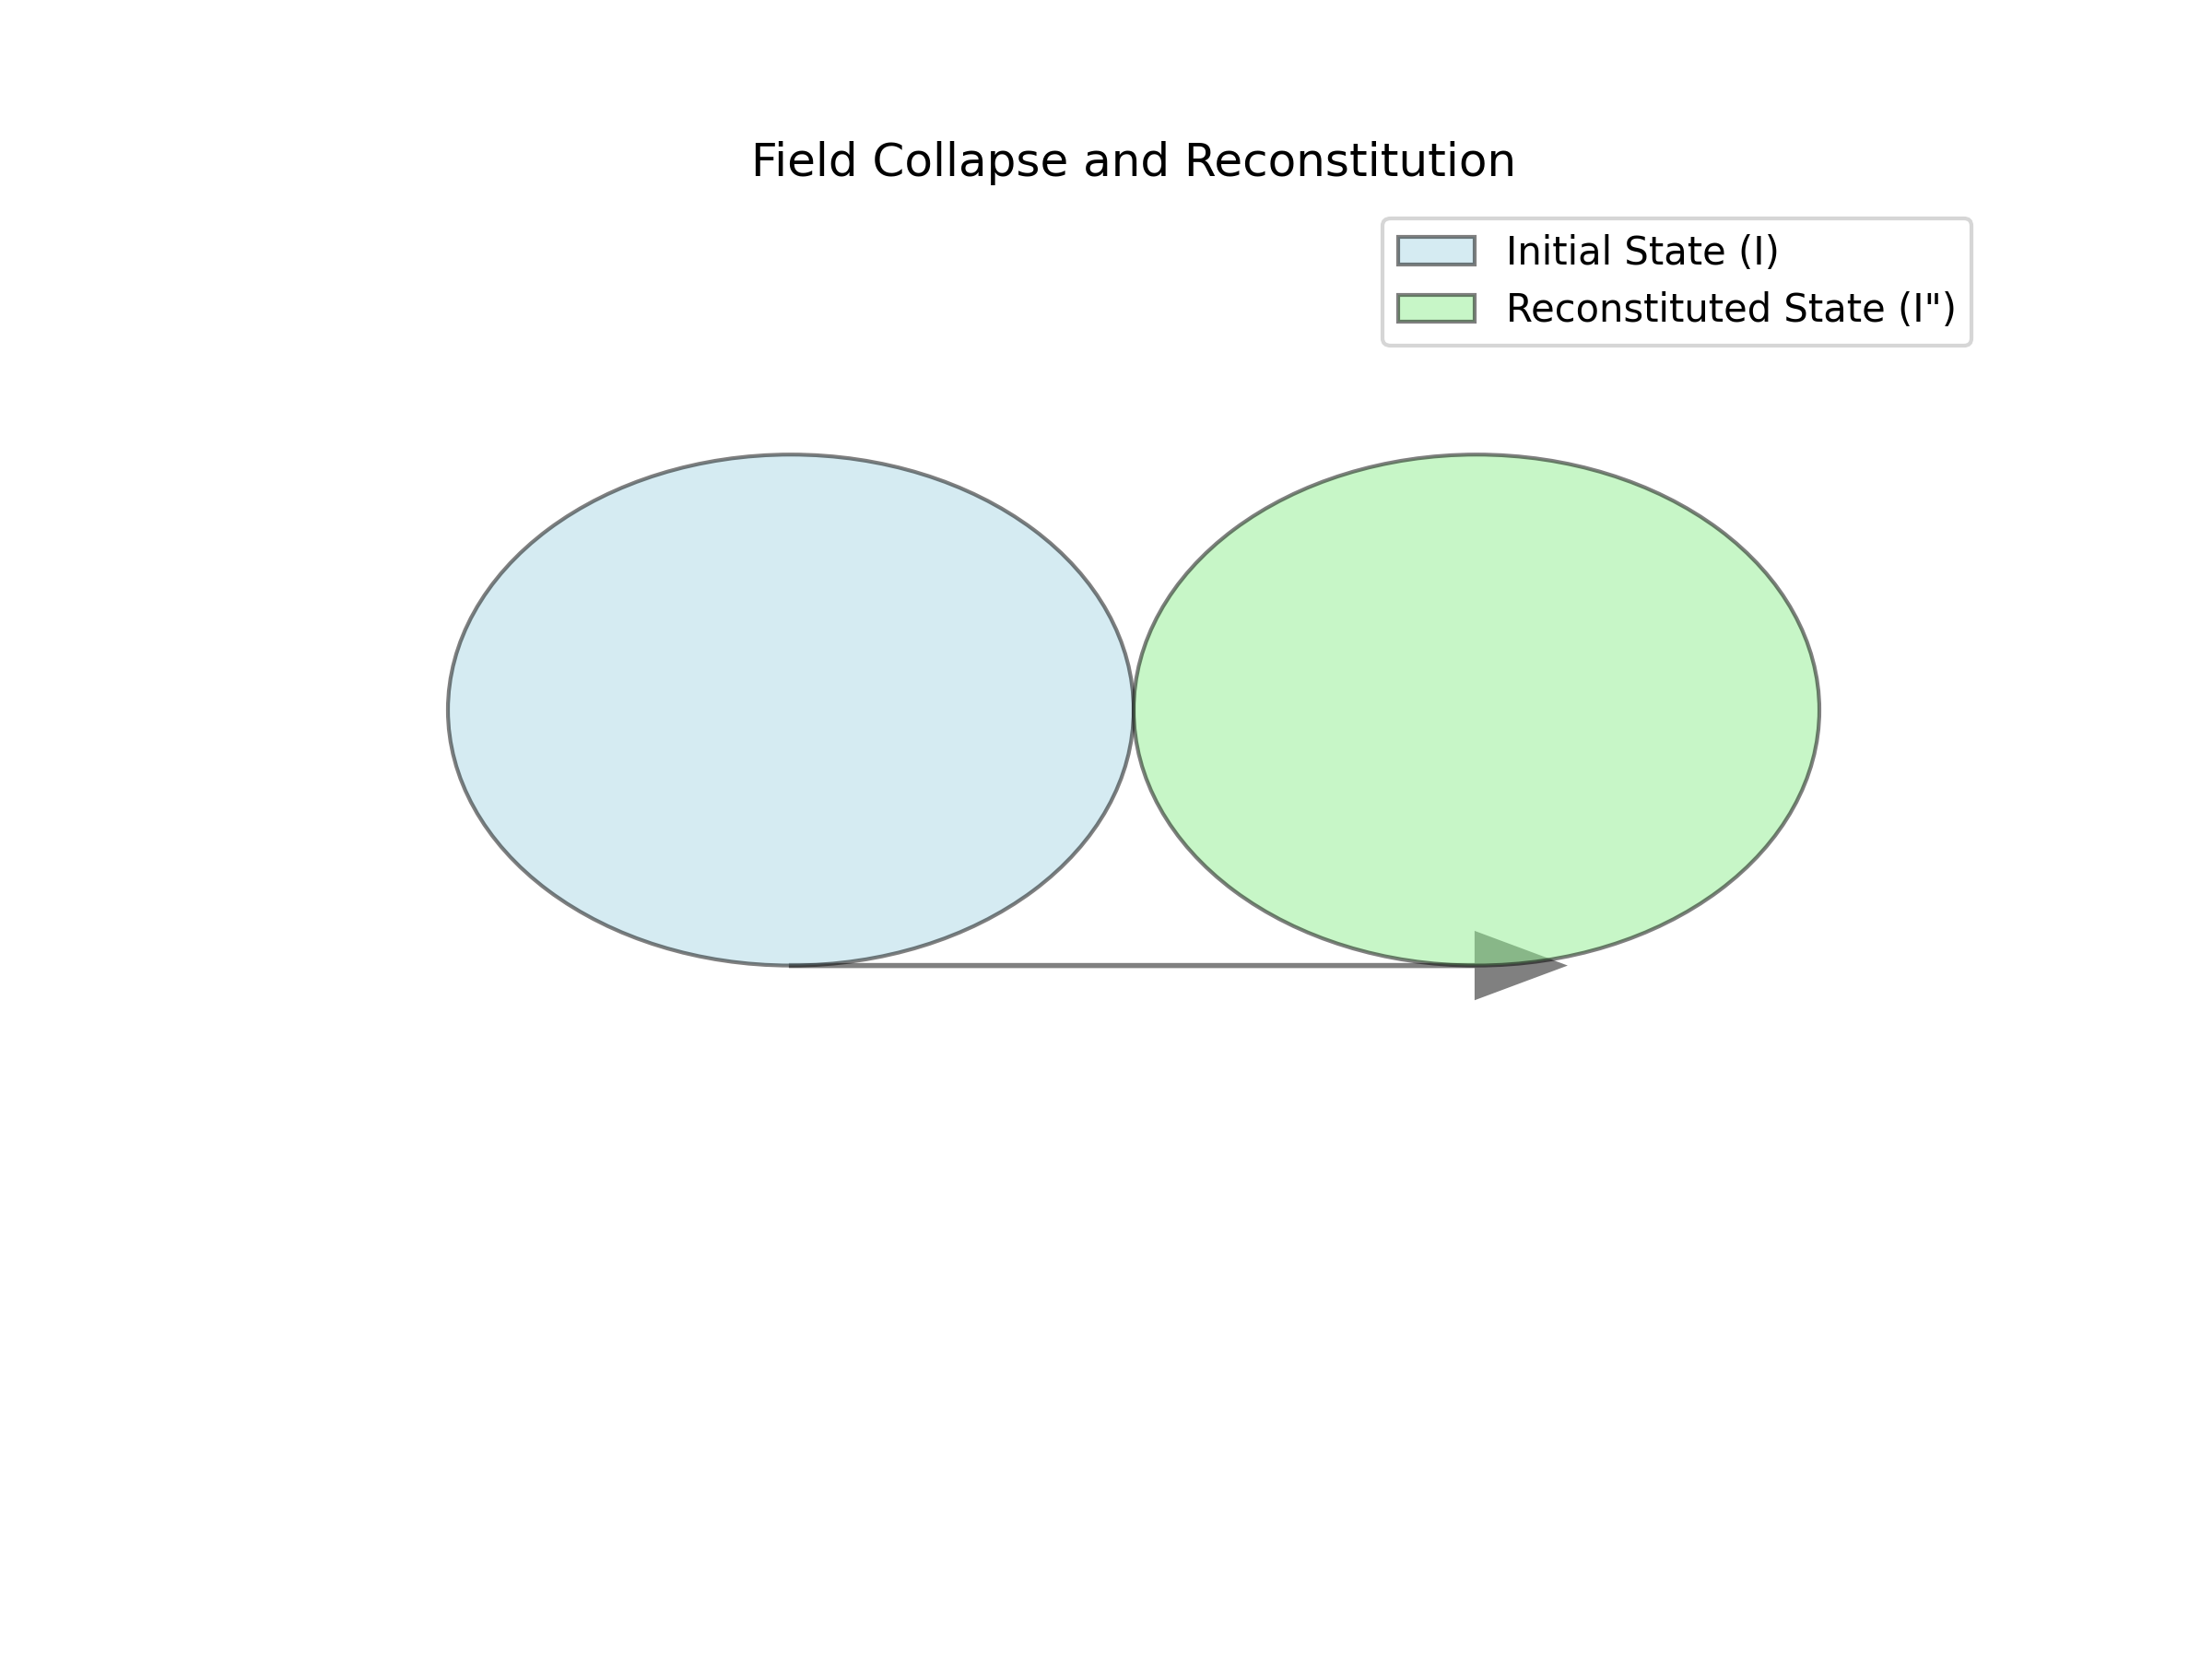
\includegraphics[width=\textwidth]{figures/ani_Field_Collapse.png}
        \caption{Field Collapse and Reconstitution: This figure illustrates the process of field collapse and subsequent reconstitution around a new axiomatic framework. The initial state (I) is depicted as a stable configuration that undergoes a collapse, leading to a reconstituted state (I'). The arrow indicates the transition from the initial to the reconstituted state, highlighting the dynamic nature of axiomatic realignment.}
        \label{fig:field_collapse}
    \end{subfigure}
    \hfill
    \begin{subfigure}[b]{0.45\textwidth}
        \centering
        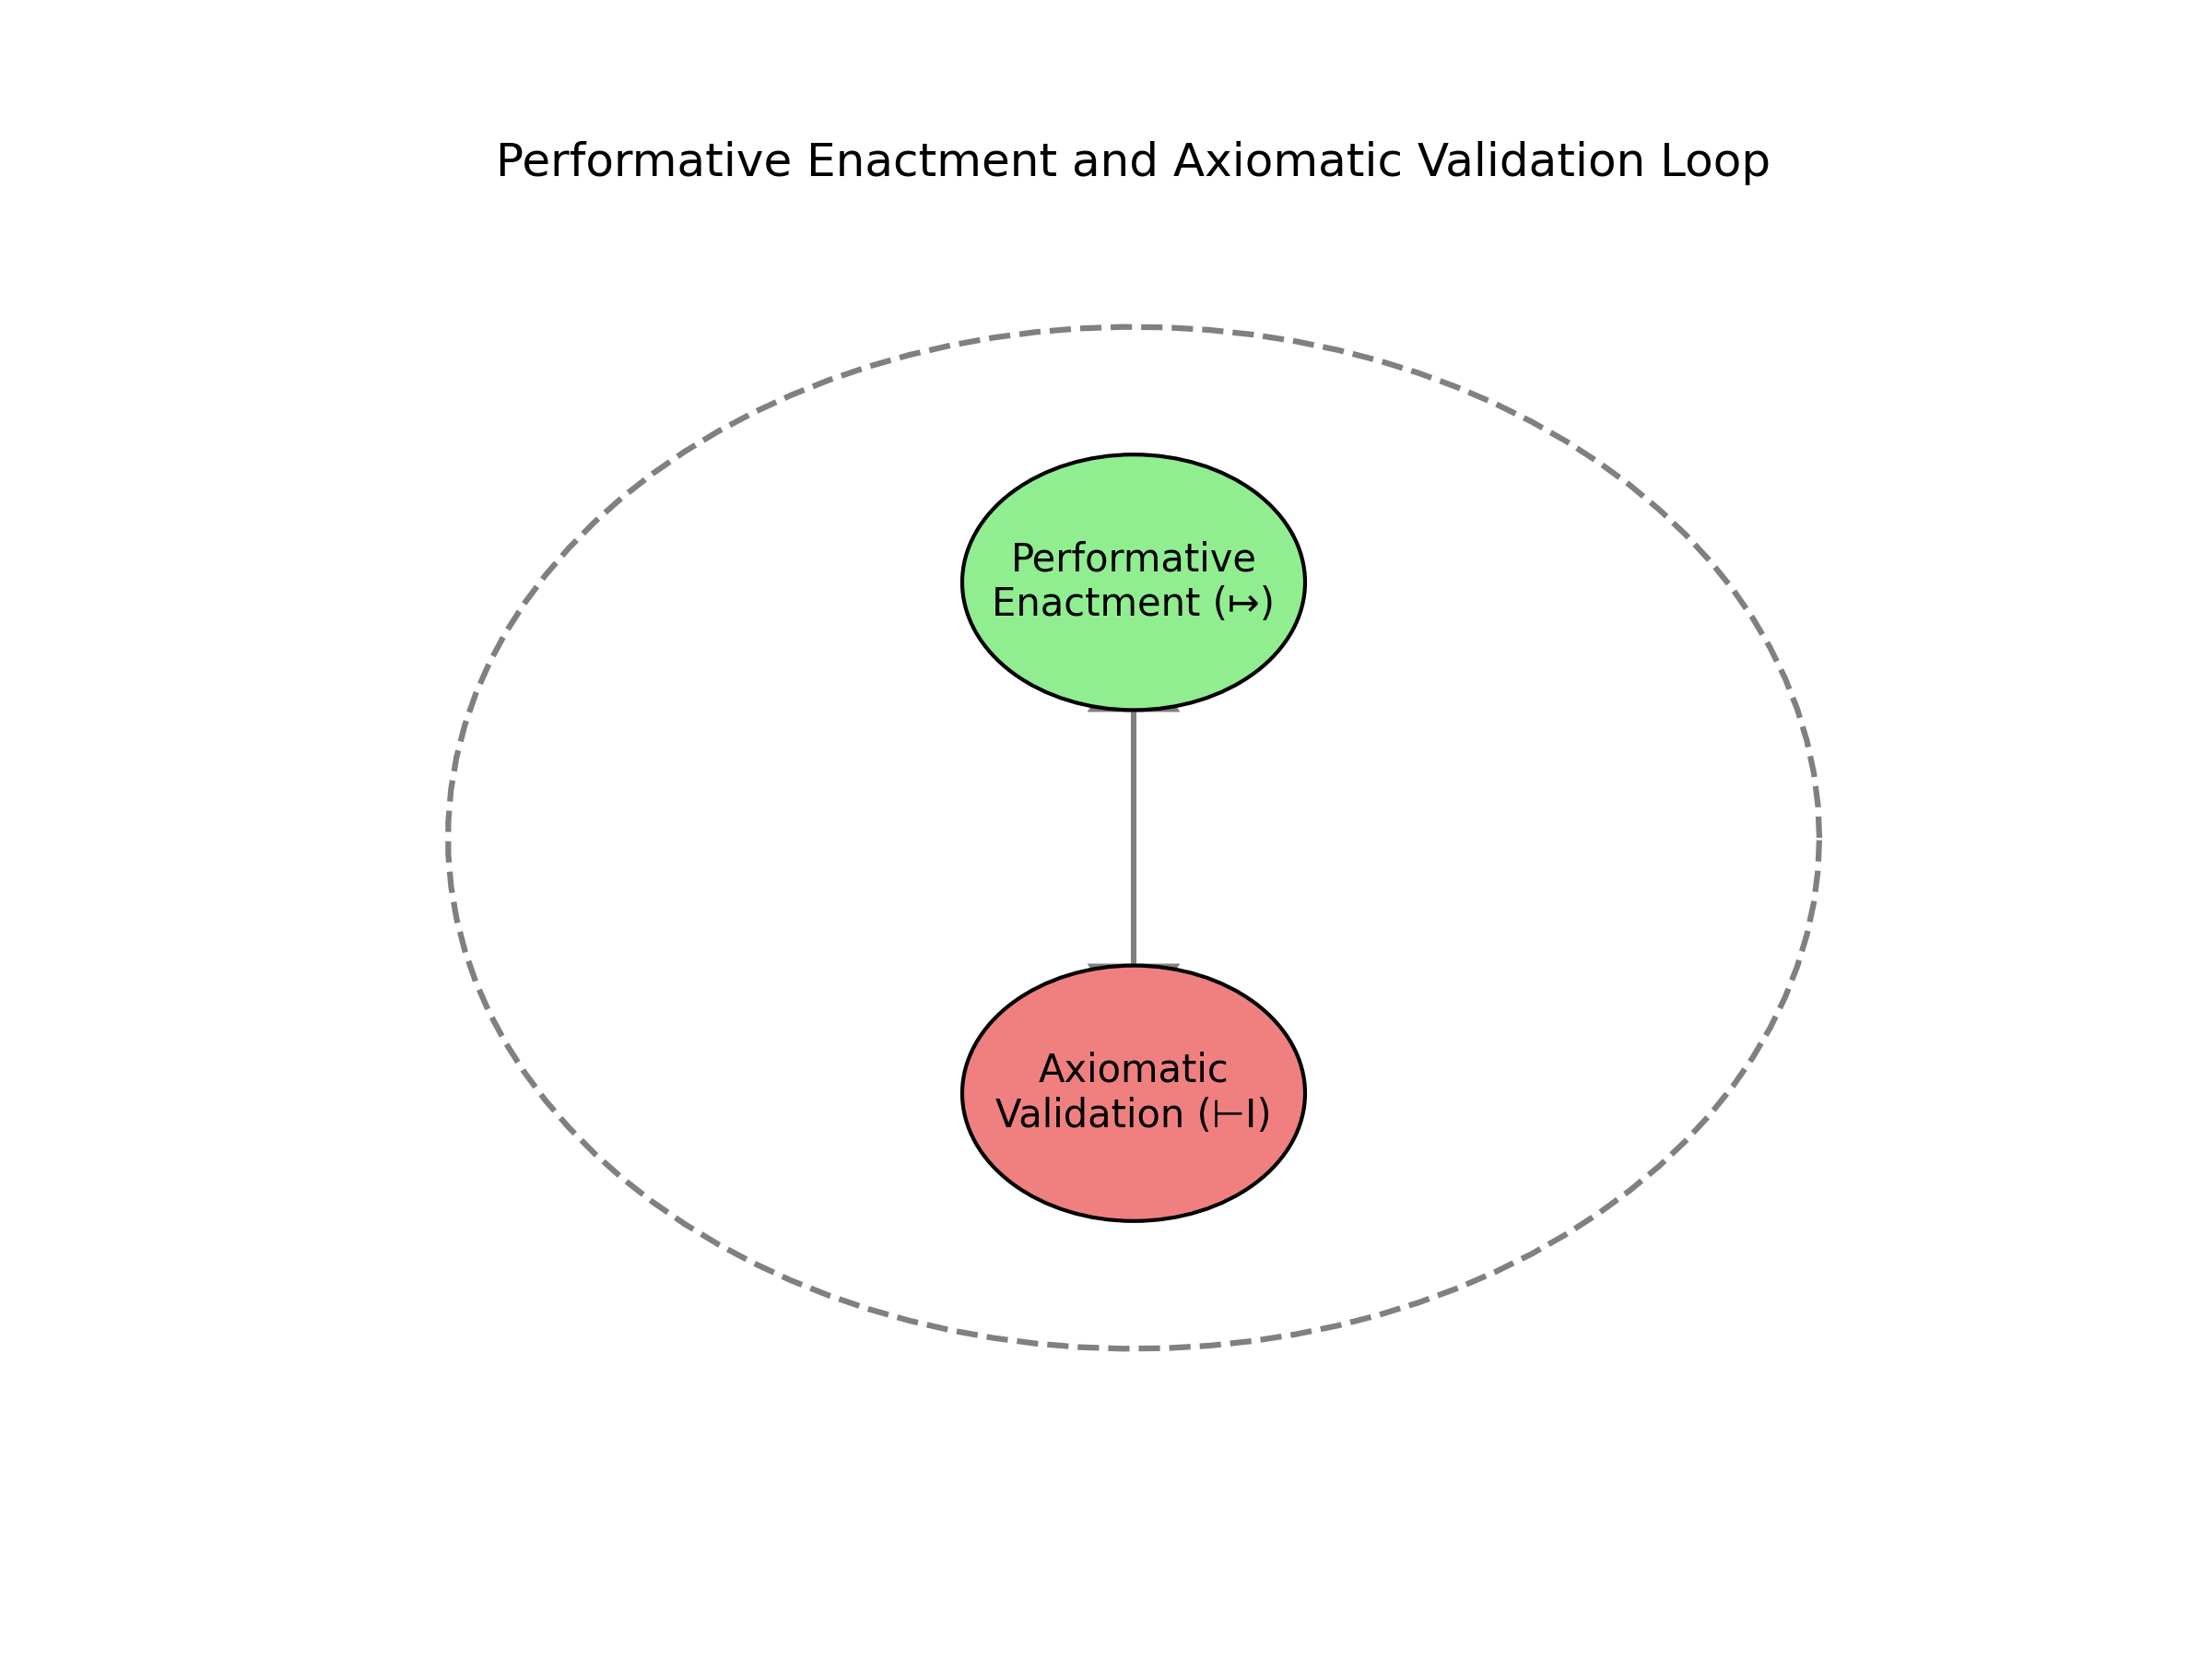
\includegraphics[width=\textwidth]{figures/ani_Performative_Enactment.png}
        \caption{Performative Enactment and Axiomatic Validation Loop: This figure depicts the core reproductive loop where performative enactment ($\mapsto$) and axiomatic validation ($\vdash_I$) reinforce the stability of the system. The circular loop represents the continuous process of enactment and validation, with arrows indicating the direction of influence between these two components.}
        \label{fig:enactment_validation}
    \end{subfigure}
    \caption{Diagrams illustrating the dynamics of field collapse and reconstitution, and the performative enactment and axiomatic validation loop within the ANI framework.}
    \label{fig:combined_1}
\end{figure}

\subsection{Fundamental Situation States: The $\orientation{\Inness}{\Isness}{\Outness}$ and $\orientation{\Outness}{\Isness}{\Inness}$ Orientations}

These structurally generated perceptual modalities dictate how reality \textit{appears}:
\begin{itemize}
    \item \textbf{$\orientation{\Inness}{\Isness}{\Outness}$:} Perception \textit{from} $\Inness$, \textit{through} $\Isness$, \textit{towards} $\Outness$. Characterized by naturalization of $\Isness$, perception of $\Outness$ as Other, focus on boundary maintenance, reinforcement of $\Inness$-group identity.
    \item \textbf{$\orientation{\Outness}{\Isness}{\Inness}$:} Perception \textit{from} $\Outness$ (or $\boundary{\Isness}$), \textit{towards} $\Isness$ and $\Inness$. Often involves denaturalization of $\Isness$, critical awareness of power/exclusion, perception of $\Inness$ as conformist/hegemonic, focus on marginalization/resistance. Dynamics between these states are key to intergroup relations.
\end{itemize}

\subsection{Axial Realignments and Ontological Inversion Events}

\ANI{} accounts for rapid reconfigurations (\textbf{Figure \ref{fig:inversion}}) where $\Inness$ and $\Outness$ positions reverse:
\begin{itemize}
    \item \textbf{Catastrophic Boundary Transgression:} Act $A'''(p) \validates{\Isness} \text{Invalid} \rightarrow A'''(p) \enactment \Outness$. Sudden shift $\orientation{\Inness}{\Isness}{\Outness} \rightarrow \orientation{\Outness}{\Isness}{\Inness}$.
    \item \textbf{Accelerated Assimilation/Conversion:} Intense enactment $\enactment$ receives powerful validation $\validates{\Isness} \text{Valid} \rightarrow$ Rapid shift $\orientation{\Outness}{\Isness}{\Inness} \rightarrow \orientation{\Inness}{\Isness}{\Outness}$.
    \item \textbf{Field Collapse and Reconstitution ($\Isness \rightarrow \Isness'$):} Catastrophic loss of coherence in $\Isness$ dissolves the triad, leading to widespread realignment upon reconstitution around $\Isness'$. Often accompanied by phenomena resembling severe cognitive dissonance \citep{Festinger1956}.
\end{itemize}
These events, marked by phenomenological disorientation, underscore the power of $\Isness$ and the volatility of validation under pressure.

% --- FIGURE 5 Integrated (Updated path) ---
\begin{figure}[h!] % Use [h!] for "here if possible, definitely!"
    \centering
    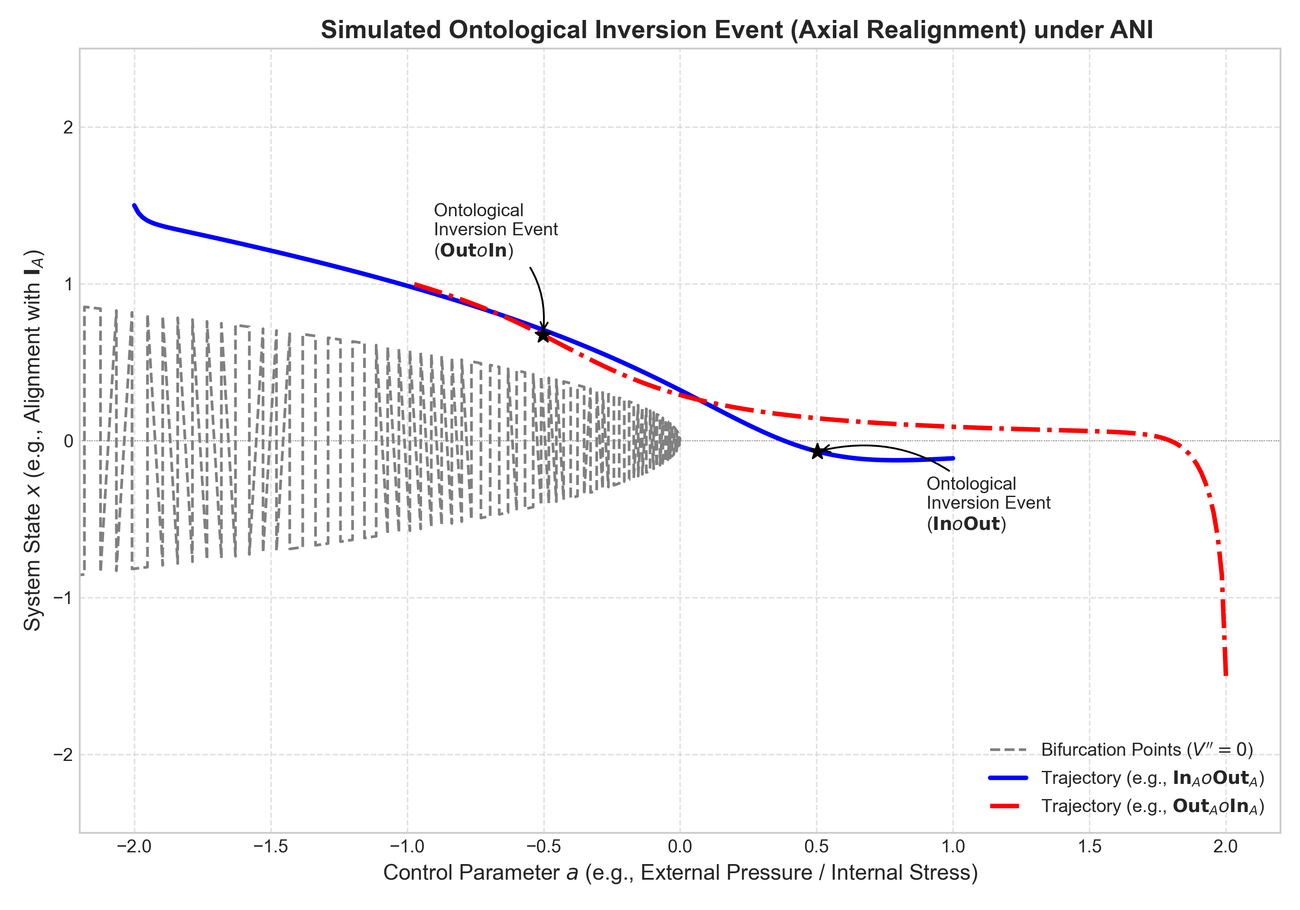
\includegraphics[width=0.9\textwidth]{figures/ani_figure4_inversion_event.png}
    \caption{Simulated Ontological Inversion Event (Axial Realignment) under ANI. Illustrates how shifts in a control parameter (\(a\), e.g., external pressure or internal axiomatic stress) can drive a system trajectory (blue/red lines representing dominant alignment with $\Inness_A$ or $\Outness_A$ relative to $\Isness_A$) across bifurcation points (dashed grey lines, V''=0). This triggers abrupt, non-linear transitions between states, modeling the dynamics of Ontological Inversion Events (e.g., $\Outness \rightarrow \Inness$, $\Inness \rightarrow \Outness$) characteristic of Axial Realignments during periods of high axiomatic flux (cf. Sec 3.4, Addendum D).}
    \label{fig:inversion}
\end{figure}

\subsection{Performative Enactment ($\enactment$) and Axiomatic Validation ($\validates{\Isness}$): The Engine of Reproduction}

Stability is achieved via ceaseless activity \citep{Goffman1959} driven by two operators:
\begin{itemize}
    \item \textbf{Performative Enactment ($\enactment$):} Actions (A), utterances, practices (P) by subjects (p) position them relative to $\Isness$ and reproduce it (e.g., $p \in \Inness$: $A(p) \enactment \Inness$; deviant $A'(p) \enactment \boundary{\Isness}$; challenging $A''(p) \enactment \Outness$).
    \item \textbf{Axiomatic Validation ($\validates{\Isness}$):} Internal logic gate assessing consistency with $\Isness$. $X \validates{\Isness} \text{Valid}$ reinforces $\Isness$; $X \validates{\Isness} \text{Invalid}$ signals deviation/exclusion.
\end{itemize}

% --- FIGURE 3 Integrated (Updated path) ---
\begin{figure}[h!]
    \centering
    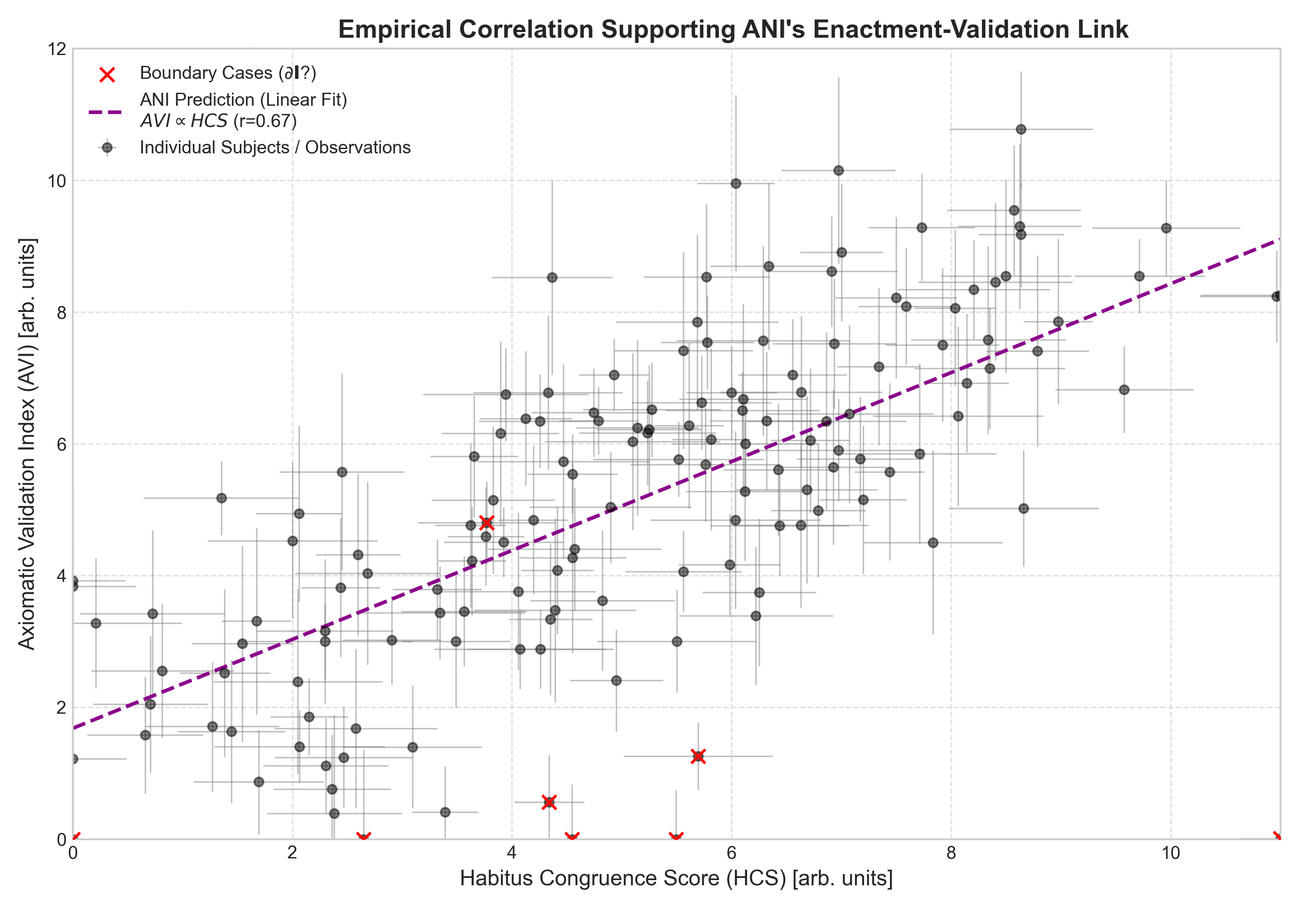
\includegraphics[width=0.9\textwidth]{figures/ani_figure3_correlation_inspired.png}
    \caption{Simulated Empirical Correlation Supporting ANI's Enactment-Validation Link. Illustrates the fundamental positive relationship between performative alignment ('Habitus Congruence Score', HCS, arb. units) and validation likelihood ('Axiomatic Validation Index', AVI, arb. units) within an \ANI{}-structured field. Data points represent individual subjects/observations with simulated measurement uncertainty. The strong linear trend (\(r=0.67\), dashed line) provides quantitative confirmation of the core nexus where \( \text{AVI} \propto \text{HCS} \). Scatter and boundary cases (red 'x', potentially representing subjects near $\boundary{\Isness}$) reflect real-world performative nuance and validation complexities entirely consistent with \ANI{} principles.}
    \label{fig:correlation}
\end{figure}

These operators form a recursive loop: Enactment sustains $\Isness \rightarrow \Isness$ provides validation framework $\validates{\Isness} \rightarrow$ Validation guides subsequent enactment. This is the engine of reproduction \citep{Bourdieu1990}, whose emergent properties are further visualized below.

% --- FIGURE 2 Integrated (Updated path) ---
\begin{figure}[h!]
    \centering
    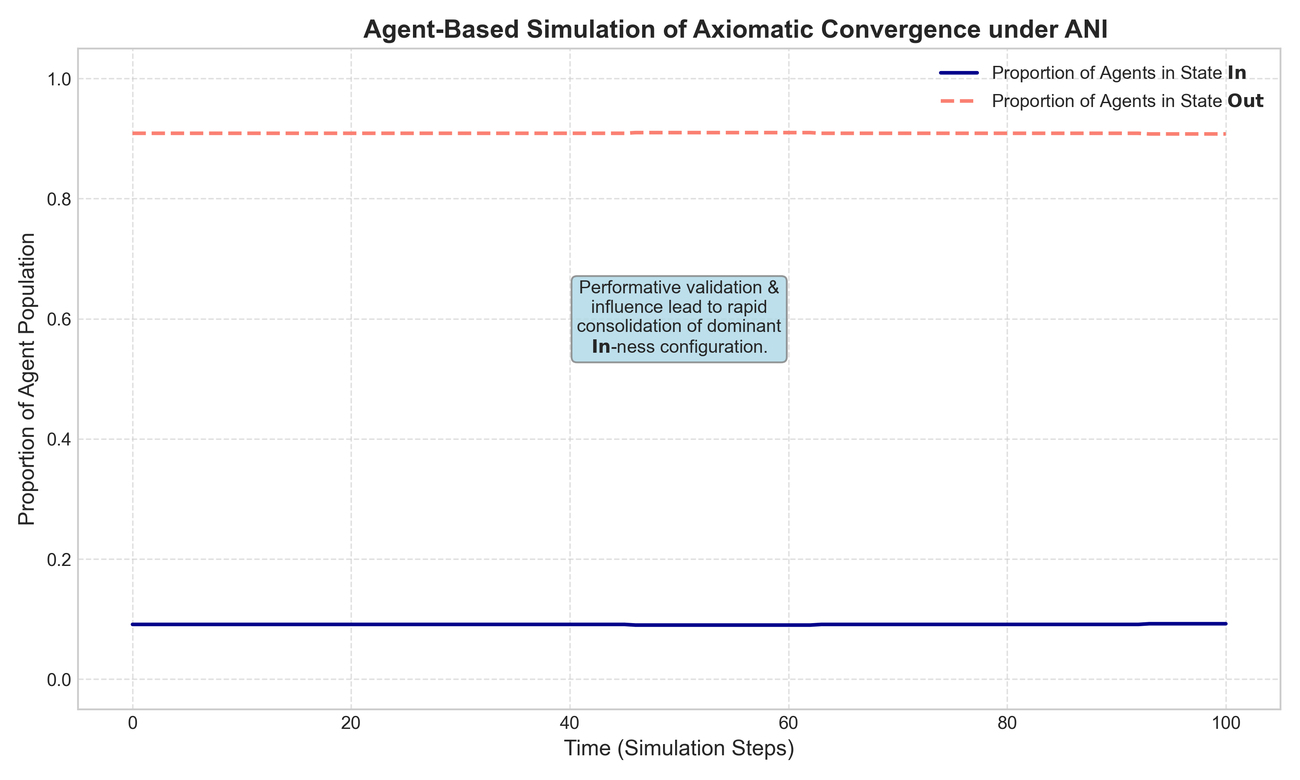
\includegraphics[width=\textwidth]{figures/ani_figure2_abm_convergence.png}
    \caption{Simulated Trajectory of Axiomatic Convergence under ANI (with Doubting State). Agent-based simulation demonstrating the emergence of stable socio-cultural order from local interactions governed by \ANI{} principles (N=2500 agents, nearest-neighbor validation influence). (a) Initial random state assignment (t=0). (b) Consolidation phase (t=200) shows emergent regions of $\Inness$ (State In, blue) and $\Outness$ (State Out, red) separated by boundary/doubting states ($\boundary{\Isness}$, yellow). (c) Near convergence (t=2000) reveals stable, large-scale axiomatic domains resulting from iterated performative validation, confirming \ANI{}'s structure-generating capacity.}
    \label{fig:convergence_grids}
\end{figure}

\subsection{The Formal Dynamics and Diagrammatic Representation}

The core reproductive loop:
\begin{enumerate}
    \item $\forall p \in \Inness$: $E[A(p), P(p)] \enactment \Inness$
    \item $\forall X \text{ arising within } \Isness$: $[X \validates{\Isness} \text{Valid}] \Rightarrow \text{Reinforces } \Isness$
    \item Guidance: $[X \validates{\Isness} \text{Valid}]$ influences future $E$.
    \item Boundary Maintenance: $A'(p) \enactment \boundary{\Isness}$; $A''(p) \enactment \Outness$. Challenges $X' \validates{\Isness} \text{Invalid}$.
\end{enumerate}

This dynamic is captured in Figure \ref{fig:ani_cycle}.

% --- FIGURE 1 Integrated (Updated path) ---
\begin{figure}[h!]
    \centering
    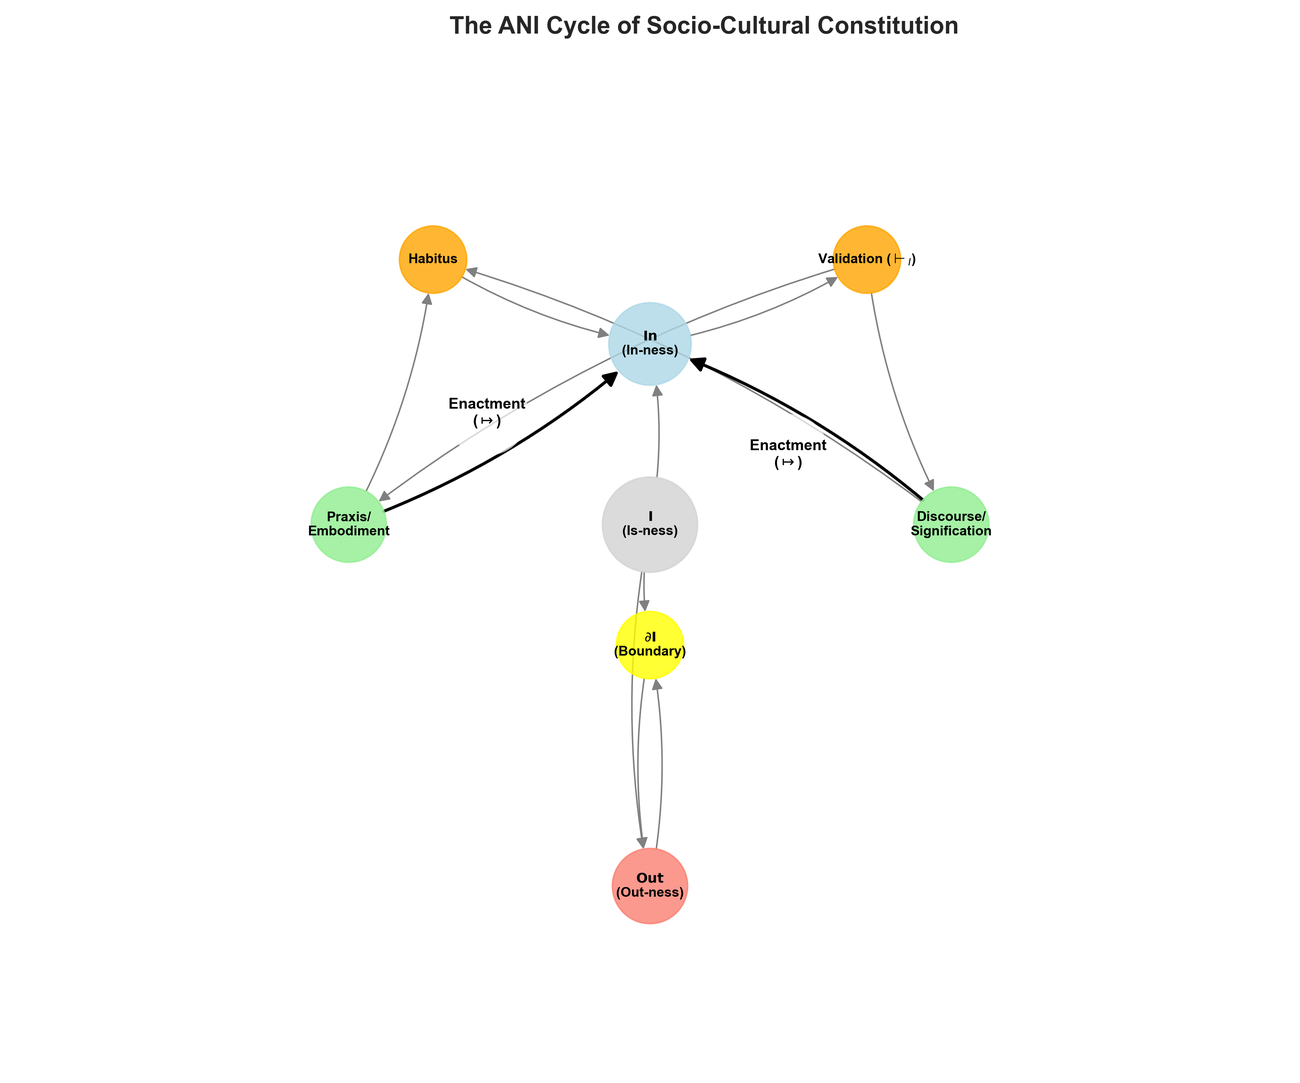
\includegraphics[width=0.8\textwidth]{figures/ani_figure1_cycle_diagram.png}
    \caption{The ANI Cycle of Socio-Cultural Constitution. Schematic representation of the recursive dynamics maintaining Is-ness ($\Isness$). Performative enactment ($\enactment$) by subjects within $\Inness$ sustains $\Isness$. $\Isness$ provides the framework for Axiomatic Validation ($\validates{\Isness}$), which guides future enactment and maintains the boundary ($\boundary{\Isness}$) separating $\Inness$ from $\Outness$. Embedded concepts (Discourse, Habitus etc.) are shown as components structured by the overarching \ANI{} logic.}
    \label{fig:ani_cycle}
\end{figure}

\section{Methodological Considerations: Apprehending the Axiomatic}

The nature of \ANI{} demands specific methodological orientations \citep{DenzinLincoln2011}.

\subsection{The Imperative of Qualitative Inquiry}

Apprehending $\Isness$, $\Inness$, $\Outness$, $\validates{\Isness}$, $\enactment$, and the $\orientation{\cdot}{\cdot}{\cdot}$ orientations requires depth, context, and meaning prioritized over measurement. Key approaches: Ethnographic Immersion (attuned to $\validates{\Isness}$) \citep{Geertz1973}, Critical Discourse Analysis (revealing axiomatic presuppositions) \citep{Foucault1972}, Phenomenological Interviewing (exploring situated perspectives) \citep{Schutz1967}, Genealogical Analysis (tracing $\Isness \rightarrow \Isness'$) \citep{Foucault1970}.

\subsection{The Ontological Mismatch of Uninformed Quantification}

Quantitative methods, \textit{when used in isolation or without qualitative grounding}, are inherently incapable of independently apprehending the axiomatic quality of $\Isness$ or the nuances of performative validation ($\validates{\Isness}$). Their reliance on pre-defined variables, aggregation, objectivist detachment, and focus on variance creates an \textit{ontological mismatch}. They cannot intrinsically "know" the axioms of $\Isness$ required to distinguish $\Inness$ from $\Outness$, nor capture the \textit{process} of $\validates{\Isness}$. Attempting to measure $\Isness$ or $\Inness$ directly via surveys misunderstands their ontological status \citep{Bourdieu1990}. However, once qualitatively informed, specific quantitative instruments or models \textit{can} be designed to track the \textit{outcomes} or \textit{correlates} of \ANI{} dynamics (as suggested by Fig \ref{fig:correlation}), serving a secondary, illustrative, or predictive-exploratory role (see Section \ref{sec:modeling}).

\subsection{Researcher Positionality}

Rigorous reflexivity regarding the researcher's own $\orientation{\Inness}{\Isness}{\Outness}$ or $\orientation{\Outness}{\Isness}{\Inness}$ position relative to the field under study is not a flaw, but a critical resource and ethical necessity \citep{Bourdieu1990}.

\section{Case Studies Illustrating ANI}

The theoretical architecture of the Axiomatic Nature of Is-ness (\ANI{}), including the fundamental Is-In-Out triad, provides a powerful analytical lens for interrogating concrete socio-cultural phenomena. While the ubiquitous nature of Is-ness ($\Isness$) means \ANI{} operates constantly across all social domains, focused case studies allow for a detailed examination of its mechanisms—performative enactment ($\enactment$), axiomatic validation ($\validates{\Isness}$), boundary work ($\boundary{\Isness}$), and the structurally generated perceptual orientations ($\orientation{\Inness}{\Isness}{\Outness}$, $\orientation{\Outness}{\Isness}{\Inness}$). The following brief illustrations demonstrate \ANI{}'s explanatory purchase.

% --- Fully Corrected Case Studies Section ---

\subsection{Case Illustration A: Coffee Break Rituals in 'Acme Corp' - Reinforcing Professional Is-ness}

\begin{itemize}
    \item \textbf{Context:} Observations conducted (hypothetically, via ethnographic immersion) within the marketing department of a mid-sized corporation, 'Acme Corp', focusing on informal coffee break interactions.
    \item \textbf{The Dominant Is-ness ($\Isness_{\text{Acme}}$):} The $\Isness$ of this department emphasizes rapid innovation, aggressive market positioning, data-driven decision-making (or the performance thereof), and a specific jargon blending marketing buzzwords with internal acronyms. Value is placed on projecting confidence and proactive engagement.
    \item \textbf{Performative Enactment ($\enactment$) and In-ness ($\Inness_{\text{Acme}}$):} Employees embodying $\Inness_{\text{Acme}}$ performatively enact $\Isness_{\text{Acme}}$ during coffee breaks. They discuss recent campaigns using the approved jargon, propose solutions framed in terms of market share or ROI, reference internal metrics (even casually), and adopt postures of focused energy. Complaining is framed constructively ("How can we overcome X challenge?"). Successful enactment (e.g., $A(p)$: pitching a jargon-laden idea; $P(p)$: displaying confident body language while holding coffee) results in $A(p), P(p) \enactment \Inness_{\text{Acme}}$, reinforcing the actor's belonging.
    \item \textbf{Axiomatic Validation ($\validates{\Isness_{\text{Acme}}}$):} Interactions are implicitly validated against $\Isness_{\text{Acme}}$. Ideas aligned with the dominant discourse receive nods, verbal affirmations ("Good point," "Exactly"), or are built upon by others ($X \validates{\Isness_{\text{Acme}}} \text{Valid}$). Conversely, remarks perceived as negative, overly critical without solutions, lacking confidence, or using incorrect jargon are met with silence, subtle dismissal, or gentle correction ($X' \validates{\Isness_{\text{Acme}}} \text{Invalid}$), subtly pushing the speaker towards the boundary $\boundary{\Isness_{\text{Acme}}}$.
    \item \textbf{Constituting Out-ness ($\Outness_{\text{Acme}}$):} Subjects consistently failing these performative validations (e.g., expressing uncertainty, questioning core assumptions, failing to adopt the jargon) become subtly marginalized, marked as 'not a team player' or 'lacking drive'. Their state becomes $\Outness_{\text{Acme}}$, defined negatively against the proactive, jargon-proficient $\Inness_{\text{Acme}}$ ideal. Their perspective shifts towards $\orientation{\Outness}{\Isness_{\text{Acme}}}{\Inness}$, potentially perceiving the dominant culture as artificial or stressful.
    \item \textbf{Orientation Dynamics:} Those comfortably within $\Inness_{\text{Acme}}$ operate from $\orientation{\Inness}{\Isness_{\text{Acme}}}{\Outness}$, perhaps viewing marginalized colleagues as simply 'not cutting it', their perception filtered through the performance-oriented $\Isness_{\text{Acme}}$.
    \item \textbf{ANI Explanation:} This mundane scenario reveals the constant, micro-level work of \ANI{} \citep{Goffman1959}. The professional $\Isness$ is not merely a set of rules, but an axiomatic field performatively sustained and validated in every interaction, simultaneously defining belonging ($\Inness$) and constituting exclusion ($\Outness$). Alternative frameworks focusing purely on power structures or individual psychology would miss the crucial \textit{axiomatic validation} loop inherent in the reproduction of $\Isness_{\text{Acme}}$.
\end{itemize}

\subsection{Case Illustration B: Online Community Moderation - Policing the Boundaries of Is-ness}

\begin{itemize}
    \item \textbf{Context:} Analysis of moderation logs and public interactions (hypothetically, via digital ethnography) within a large online forum dedicated to a specific science fiction franchise, 'Oblivious Awakening X'.
    \item \textbf{The Dominant Is-ness ($\Isness_{\text{GQX}}$):} This fan community's $\Isness$ values deep lore knowledge, specific interpretive frameworks (e.g., favouring certain character arcs, debating established canon rules), adherence to community etiquette (spoiler warnings, respectful debate tone), and collective enthusiasm for the franchise.
    \item \textbf{Performative Enactment ($\enactment$) and In-ness ($\Inness_{\text{GQX}}$):} Members achieve $\Inness_{\text{GQX}}$ by posting detailed analyses referencing obscure lore, participating in established debate formats, correctly using spoiler tags, and expressing positive affect towards the franchise and fellow "true fans." $A(p)$: posting a well-argued canonical analysis; $P(p)$: using community-specific emojis appropriately $\enactment \Inness_{\text{GQX}}$.
    \item \textbf{Axiomatic Validation ($\validates{\Isness_{\text{GQX}}}$) and Boundary Work ($\boundary{\Isness_{\text{GQX}}}$):} Moderators and established users actively perform axiomatic validation. Posts demonstrating lore mastery and adherence to interpretive norms are upvoted, praised, and cited ($X \validates{\Isness_{\text{GQX}}} \text{Valid}$). Explicit boundary work occurs through moderation actions: deleting off-topic posts, correcting lore errors, warning users for violating etiquette (violations $\validates{\Isness_{\text{GQX}}} \text{Invalid}$). These actions define and police $\boundary{\Isness_{\text{GQX}}}$.
    \item \textbf{Constituting Out-ness ($\Outness_{\text{GQX}}$):} Users who persistently violate norms, display ignorance of core lore, challenge deeply held fan interpretations ("trolls"), or express negativity towards the franchise are labeled as "casuals," "haters," or are explicitly banned. They are constituted as $\Outness_{\text{GQX}}$. Their orientation becomes $\orientation{\Outness}{\Isness_{\text{GQX}}}{\Inness}$, perhaps viewing the community as gatekeeping elitists \citep{Bourdieu1984}.
    \item \textbf{Axial Realignment Potential:} A user, previously $\Inness_{\text{GQX}}$, who posts a major spoiler without warning or vehemently argues against a core community interpretation might face immediate, severe sanction ($A'''(p) \enactment \Outness_{\text{GQX}}$), experiencing an Ontological Inversion Event within this specific field.
    \item \textbf{ANI Explanation:} \ANI{} reveals online community formation not just as shared interest, but as the active constitution of an $\Isness$ through performative validation and boundary policing. The passion of fandom here provides explicit examples of axiomatic validation ($\validates{\Isness_{\text{GQX}}}$) and the construction of $\Inness/\Outness$ distinctions based on adherence to the specific $\Isness_{\text{GQX}}$. Power dynamics (moderators, established fans) are understood as roles facilitating the maintenance of $\Isness_{\text{GQX}}$.
\end{itemize}

\subsection{Case Illustration C: Cargo Cult Dynamics in Influencer Ecosystems}

\begin{itemize}
    \item \textbf{Context:} Analysis of content creation patterns, engagement metrics, and discourse within communities surrounding social media influencers (e.g., Instagram, TikTok, YouTube), drawing parallels with anthropological studies of cargo cults.
    \item \textbf{The Dominant Is-ness ($\Isness_{\text{Influence}}$):} The $\Isness$ of this sphere dictates specific aesthetic conventions, content formats (e.g., challenges, hauls, GRWM), performative authenticity strategies, algorithmic optimization tactics, and a discourse centered on growth, engagement, and monetization ('the cargo'). Success is axiomatically validated ($\validates{\Isness_{\text{Influence}}}$) through follower counts, likes, brand deals.
    \item \textbf{Performative Enactment ($\enactment$) and Ritualistic Mimicry:} Aspiring influencers (often situated initially in $\Outness_{\text{Influence}}$ or $\boundary{\Isness_{\text{Influence}}}$) engage in intense performative enactment, meticulously mimicking the styles, content, and engagement-seeking behaviors of established figures embodying $\Inness_{\text{Influence}}$. This mimicry functions as a ritualistic practice aimed at invoking the desired outcome of success, much like cargo cult rituals attempting to attract material goods (perhaps echoing structuralist analyses of myth \citep{LeviStrauss1969}?). $A(p)$: replicating a viral trend; $P(p)$: adopting a specific visual aesthetic $\enactment$ towards $\Inness_{\text{Influence}}$.
    \item \textbf{Axiomatic Validation via Algorithm and Audience:} Validation ($\validates{\Isness_{\text{Influence}}}$) is partially automated via platform algorithms (rewarding content aligned with $\Isness_{\text{Influence}}$) and audience reception (likes, shares, positive comments). Successful validation reinforces the practices and solidifies $\Inness_{\text{Influence}}$ status. Failure leads to remaining in $\Outness_{\text{Influence}}$, often accompanied by frustration or accusations of algorithmic bias (an $\orientation{\Outness}{\Isness_{\text{Influence}}}{\Inness}$ perspective).
    \item \textbf{ANI Explanation:} \ANI{} reframes the influencer economy beyond simple market dynamics. It reveals a potent $\Isness$ sustained by ritualistic performative enactment aimed at securing validation within an often opaque axiomatic system (partially governed by algorithms). The concept of the cargo cult highlights the quasi-magical thinking embedded within $\Isness_{\text{Influence}}$, where specific performances are believed to axiomatically guarantee success \citep{Festinger1956}.
\end{itemize}

\subsection{Case Illustration D: Succession Crises in Hermetic Political Systems (e.g., Politburo Dilemma)}

\begin{itemize}
    \item \textbf{Context:} Applying \ANI{} to analyze historical or hypothetical power struggles during leadership transitions within hierarchical, ideologically rigid political structures like a Politburo.
    \item \textbf{The Dominant Is-ness ($\Isness_{\text{Politburo}}$):} This $\Isness$ comprises official party ideology, complex unwritten rules of seniority and factional maneuvering, prescribed rhetorical styles, historical narratives legitimizing the current order, and intense suspicion of deviation. Loyalty (or its performance) is paramount.
    \item \textbf{High-Stakes Performative Enactment ($\enactment$) and In-ness ($\Inness_{\text{Politburo}}$):} During succession crises, actors vying for power or survival engage in heightened performative enactment. $A(p)$: delivering ideologically pure speeches; $P(p)$: strategically aligning with powerful factions; careful displays of deference or authority $\enactment \Inness_{\text{Politburo}}$ (or maintenance thereof). The stakes are incredibly high, as validation determines access to ultimate power.
    \item \textbf{Axiomatic Validation ($\validates{\Isness_{\text{Politburo}}}$) by Inner Circle:} Validation is performed by the core elite who embody and control $\Isness_{\text{Politburo}}$. Endorsements, appointments, control over security apparatuses, and manipulation of official narratives function as $\validates{\Isness_{\text{Politburo}}} \text{Valid}$. Denunciations, purges, or historical revisionism function as $\validates{\Isness_{\text{Politburo}}} \text{Invalid}$.
    \item \textbf{Ontological Inversion Events:} Succession crises are fertile ground for Axial Realignments. A previously powerful figure ($\Inness_{\text{Politburo}}$) can be suddenly denounced and purged ($A'''(p) \enactment \Outness_{\text{Politburo}}$), experiencing a catastrophic inversion. Conversely, a dark horse candidate might rapidly consolidate power through successful enactment and validation, achieving supreme $\Inness_{\text{Politburo}}$. The $\orientation{\Inness}{\Isness_{\text{Politburo}}}{\Outness}$ perspective within this $\Isness$ is one of constant vigilance; the $\orientation{\Outness}{\Isness_{\text{Politburo}}}{\Inness}$ perspective is often one of existential threat or plotting.
    \item \textbf{ANI Explanation:} \ANI{} moves beyond standard political science models of power balancing. It emphasizes how the specific ideological and procedural $\Isness_{\text{Politburo}}$ itself structures the conflict, defining the terms of legitimate enactment and validation. The succession crisis becomes a crucible where the axiomatic force of $\Isness_{\text{Politburo}}$ is tested and ultimately reasserted, often through brutal Ontological Inversion Events \citep{Arendt1951}.
\end{itemize}

\subsection{Case Illustration E: Meta-Relevance and Memetic Propagation in the 'Digital Noosphere'}

\begin{itemize}
    \item \textbf{Context:} Analyzing the rapid creation, mutation, and dissemination of internet memes and cultural references within online spaces, conceptualized as a 'digital noosphere' \citep{Castells2000} or memetic multiverse.
    \item \textbf{The Dominant Is-ness ($\Isness_{\text{Meme}}(t)$):} This $\Isness$ is exceptionally fluid and time-dependent (denoted $\Isness_{\text{Meme}}(t)$). It consists of the currently relevant set of memes, in-jokes, cultural references, platform-specific formats, and ironic postures. $\Isness_{\text{Meme}}(t)$ defines what is considered 'current,' 'dank,' 'meta,' or conversely, 'normie,' 'cringe,' 'dead.'
    \item \textbf{Performative Enactment ($\enactment$) via Memetic Deployment:} Users achieve $\Inness_{\text{Meme}}$ by demonstrating awareness of and competence in deploying the currently validated elements of $\Isness_{\text{Meme}}(t)$. $A(p)$: correctly using a new meme format; $P(p)$: adopting the appropriate layer of irony $\enactment \Inness_{\text{Meme}}$. This enactment is often aimed at signaling cultural capital and belonging \citep{Bourdieu1984}.
    \item \textbf{Axiomatic Validation ($\validates{\Isness_{\text{Meme}}(t)}$) via Networked Reception:} Validation is rapid and distributed, occurring through likes, shares, upvotes, comments ("based," "lol"), and integration into subsequent memetic iterations ($X \validates{\Isness_{\text{Meme}}(t)} \text{Valid}$). Failure to resonate, misuse of a meme, or deploying an 'expired' reference leads to being ignored, downvoted, or mocked ($X' \validates{\Isness_{\text{Meme}}(t)} \text{Invalid}$), marking the user as lagging behind $\Isness_{\text{Meme}}(t)$ and pushing them towards $\Outness_{\text{Meme}}$.
    \item \textbf{Multiplicity and Field Collapse:} Tanaka might provocatively suggest this memetic field echoes multiverse concepts, with countless potential $\Isness$ variations constantly competing. The rapid obsolescence of memes \citep{Dawkins1976} represents frequent micro-scale 'Field Collapse and Reconstitution' ($\Isness_{\text{Meme}}(t) \rightarrow \Isness_{\text{Meme}}(t+\Delta t)$). The $\orientation{\Inness}{\Isness_{\text{Meme}}(t)}{\Outness}$ perspective is fleeting; the $\orientation{\Outness}{\Isness_{\text{Meme}}(t)}{\Inness}$ perspective ('being out of touch') is a constant threat.
    \item \textbf{ANI Explanation:} \ANI{} provides a framework for understanding memetic culture beyond simple imitation or epidemiology. It highlights the role of a rapidly shifting, axiomatically functioning $\Isness$ that dictates relevance and belonging. Performative enactment (meme creation/use) and distributed validation (networked reception) drive the system, constantly defining the boundaries of $\Inness_{\text{Meme}}$ ('being online') and $\Outness_{\text{Meme}}$ ('touching grass'), governed by the ephemeral $\Isness_{\text{Meme}}(t)$.
\end{itemize}

These illustrations, though brief, demonstrate the analytical power of \ANI{}. By focusing on the interplay of Is-ness ($\Isness$), performative enactment ($\enactment$), axiomatic validation ($\validates{\Isness}$), and the resultant Is-In-Out triad, \ANI{} provides a unified framework for understanding the constitution and reproduction of diverse socio-cultural realities, moving beyond superficial descriptions to reveal the underlying axiomatic logic at play.

\section{Theorizing Transformation: ANI and the Dynamics of Social Change}

\ANI{} provides the ontological logic for understanding transformation ($\Isness \rightarrow \Isness'$) as inherent within its framework, not a contradiction. Change confirms \ANI{}'s fundamental logic.

\subsection{Sources of Destabilization}

\ANI{} identifies endogenous/exogenous factors: Internal Axiomatic Stress (contradictions within $\Isness$), Erosion of Performative Efficacy (waning $\enactment$), Exogenous Shocks/Encounters (challenges from $\Isness'$ or material reality), Counter-Axiomatic Pressure from $\Outness$ ($\orientation{\Outness}{\Isness}{\Inness}$ challenges). These echo dynamics observed in complex adaptive systems \citep{Prigogine1984, Bateson1972}.

\begin{figure}[htbp]
    \centering
    \begin{subfigure}[b]{0.65\textwidth}
        \centering
        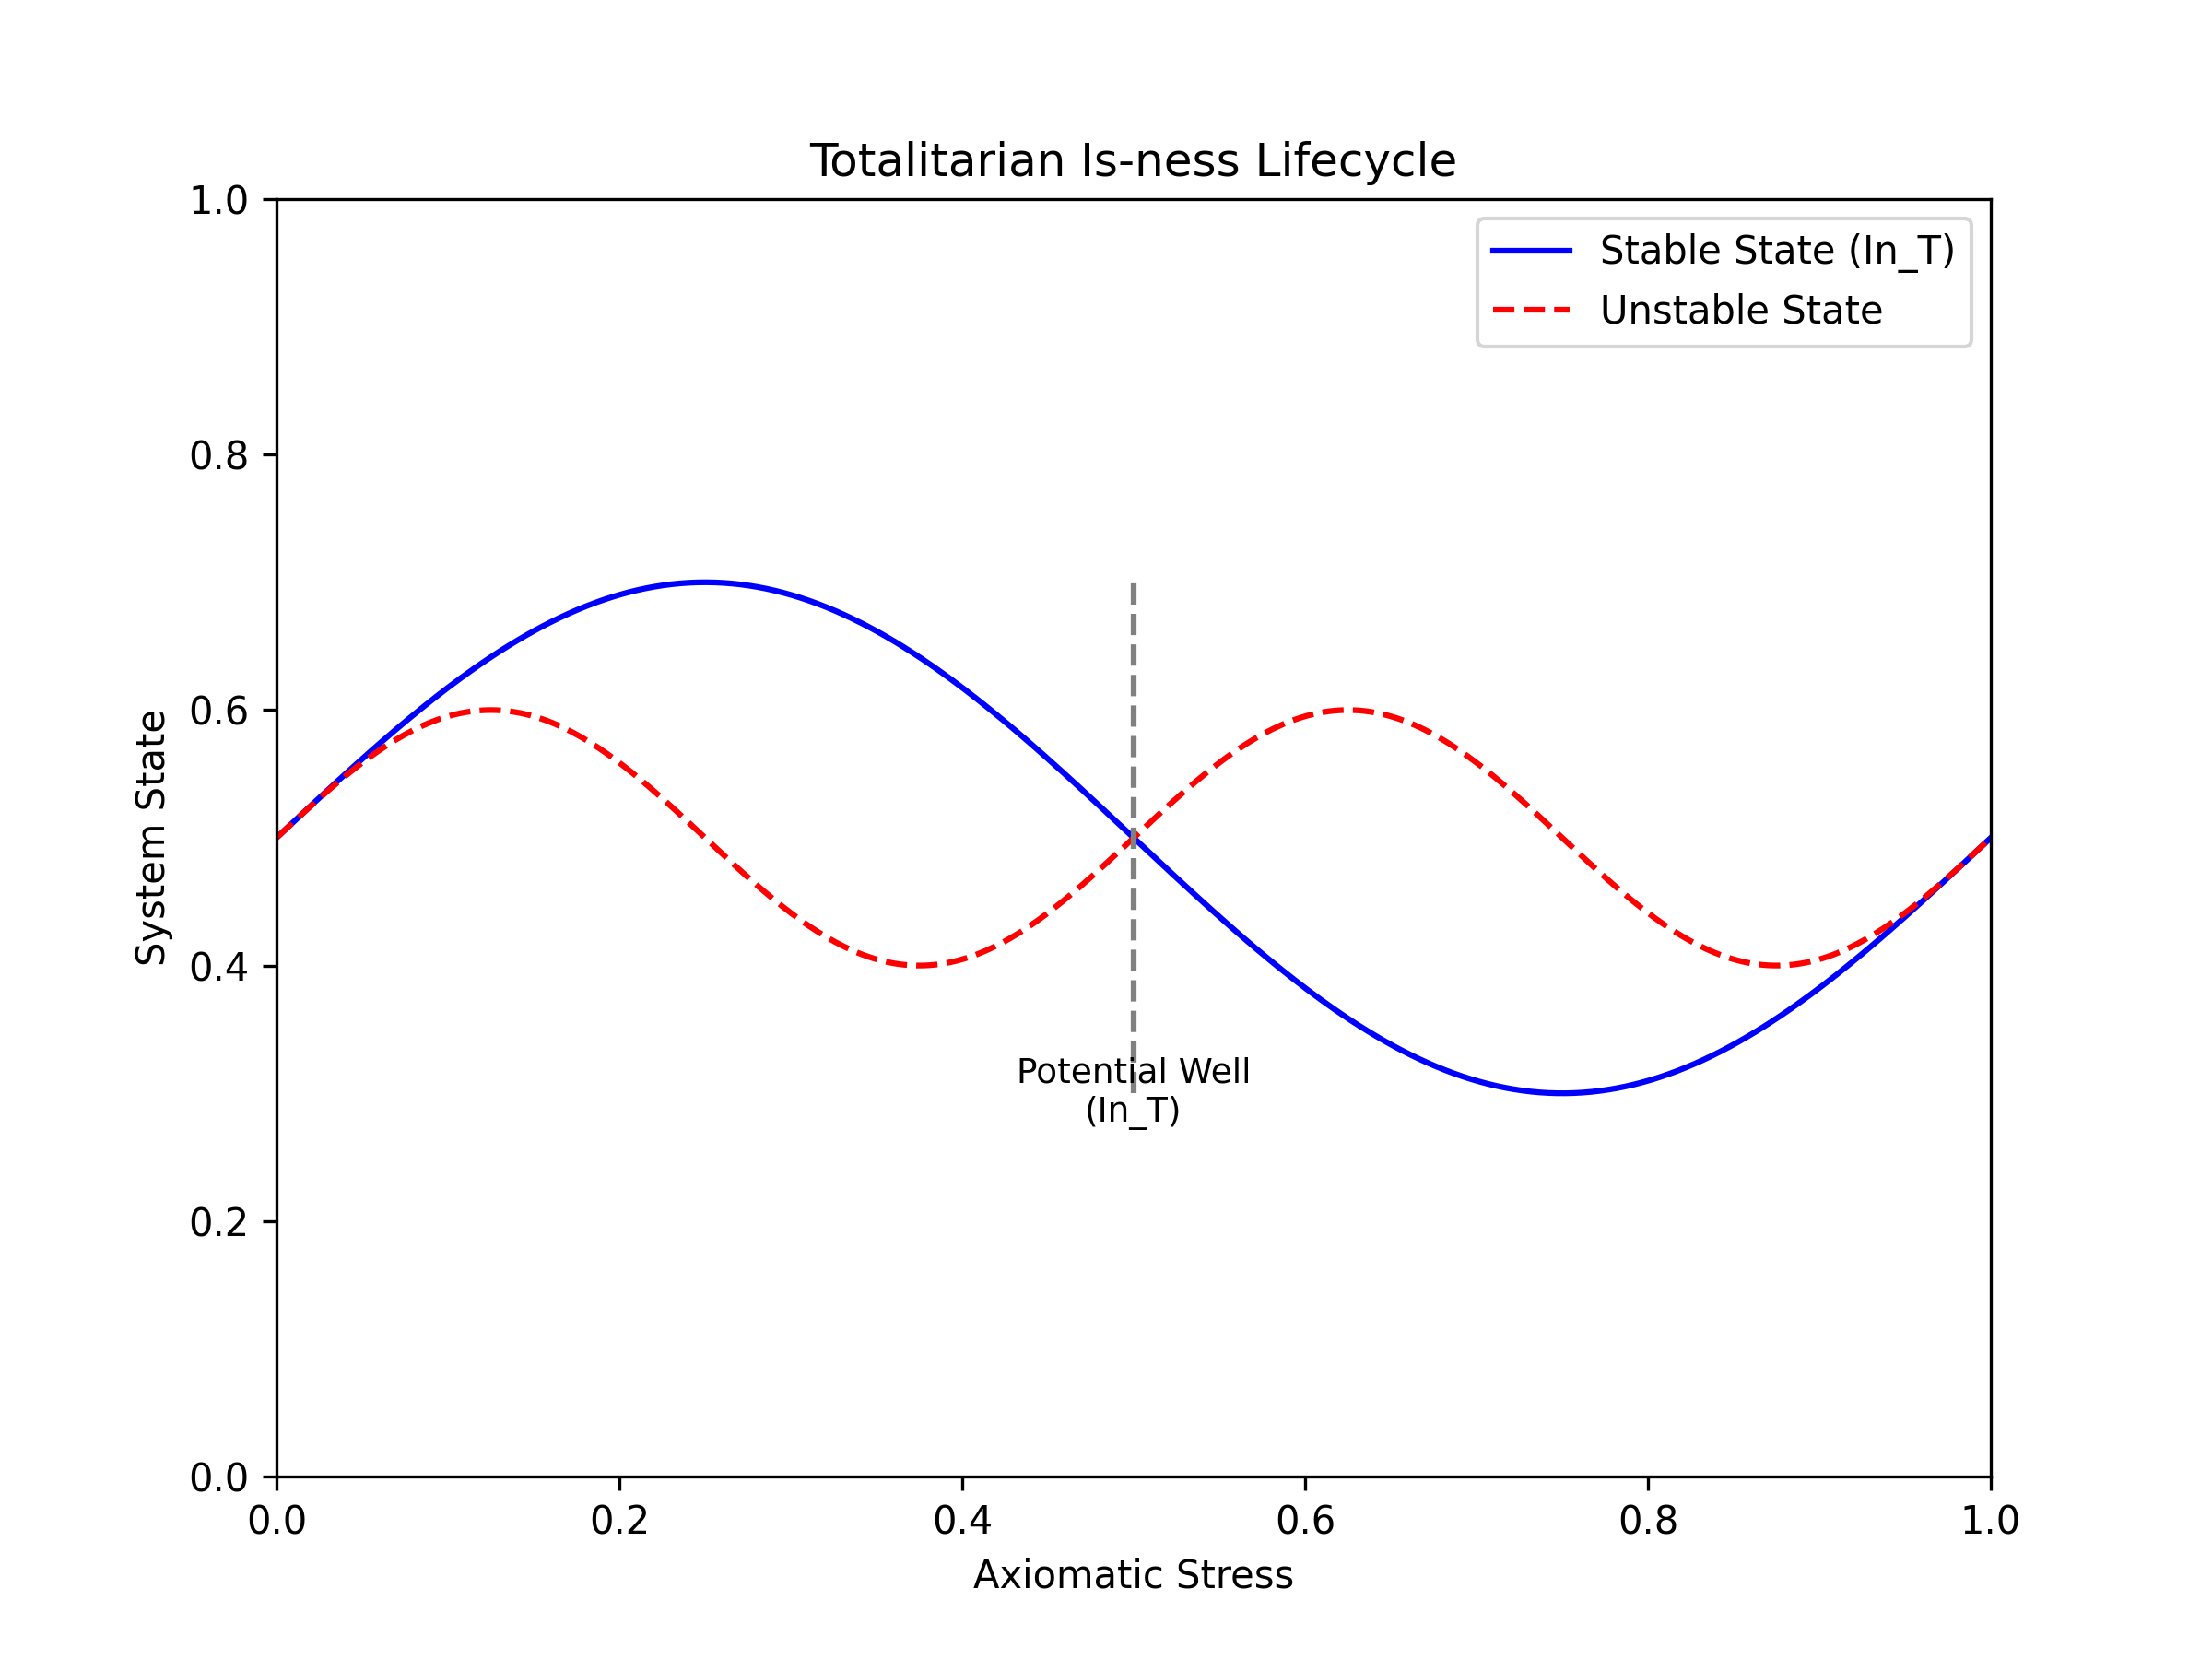
\includegraphics[width=\textwidth]{figures/ani_Totalitarian-Lifecycle.png}
        \caption{Totalitarian Is-ness Lifecycle: This phase space diagram illustrates the dynamics of a totalitarian system, showing how it can transition from a stable state to an unstable one due to increasing axiomatic stress. The blue line represents the stable state (In\_T), while the red dashed line indicates the unstable state. The potential well signifies the deep, sharp attractor that draws individuals towards the stable state.}
        \label{fig:totalitarian_lifecycle}
    \end{subfigure}
    \hfill
    \begin{subfigure}[b]{0.65\textwidth}
        \centering
        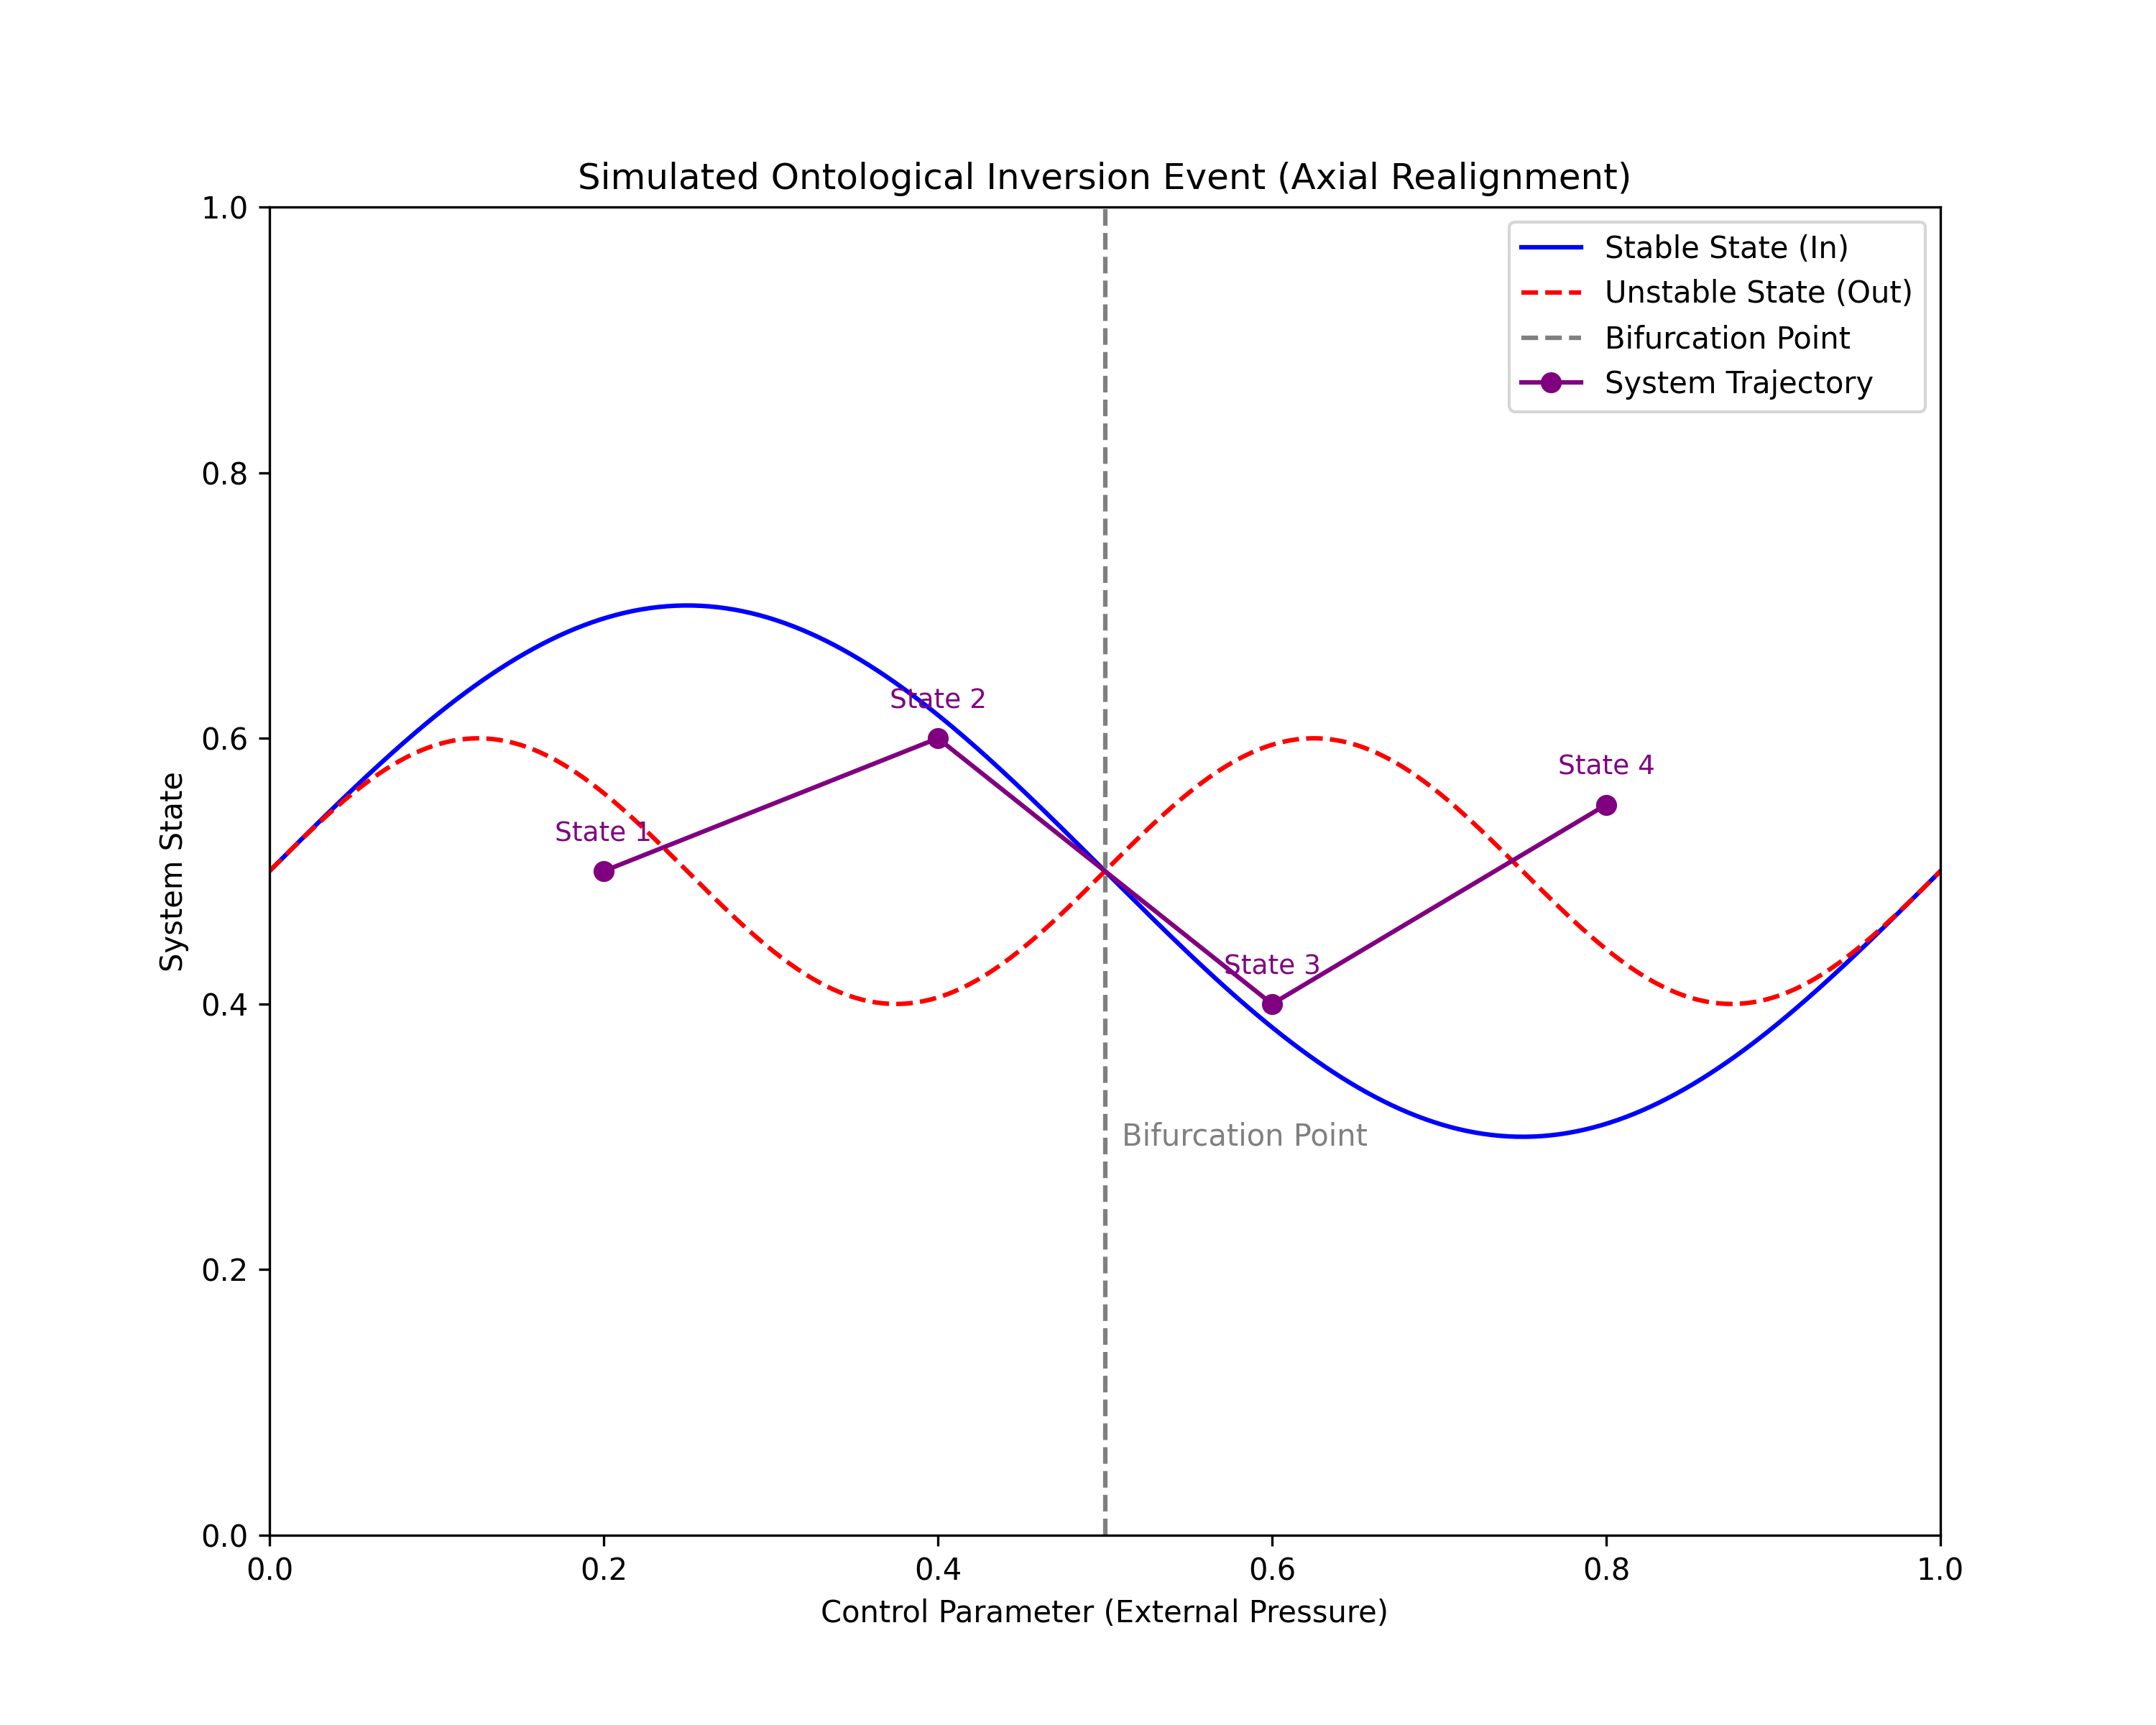
\includegraphics[width=\textwidth]{figures/ani_Ontological_Inversion.png}
        \caption{Simulated Ontological Inversion Event (Axial Realignment): This bifurcation diagram shows how shifts in a control parameter (e.g., external pressure) can drive a system trajectory across bifurcation points, triggering abrupt transitions between states representing In-ness and Out-ness relative to the governing Is-ness (I). The purple line with markers illustrates the system trajectory through different states, highlighting the path of ontological inversion.}
        \label{fig:ontological_inversion}
    \end{subfigure}
    \caption{Diagrams illustrating the totalitarian Is-ness lifecycle \ref{sec:axiomatic-extremes} and the simulated ontological inversion event within the ANI framework.}
    \label{fig:combined_2}
\end{figure}

\subsection{The Trajectory of Change: De-stabilization, Liminality, Re-Axiomatization}

Transformation follows a typical trajectory understood via \ANI{}:
\begin{enumerate}
    \item \textbf{De-stabilization:} Weakening axiomatic force of $\Isness$; $\validates{\Isness}$ becomes contested; $\enactment$ fragments; $\boundary{\Isness}$ becomes porous/contested.
    \item \textbf{Liminal Phase:} Uncertainty; competing potential Is-nesses ($\Isness'$, $\Isness''$) vie for dominance; identities fluid; conflict as groups attempt to impose preferred configurations; Ontological Inversion Events (Fig \ref{fig:inversion}) may increase.
    \item \textbf{Re-Axiomatization Phase:} Consolidation of a new or modified Is-ness ($\Isness'$) establishing its own $\validates{\Isness'}$, $\enactment'$, and $\Isness'$-$\Inness'$-$\Outness'$ triad. Stability is restored under a new axiomatic regime (cf. convergence tendency, Fig \ref{fig:convergence_grids}).
\end{enumerate}
Change is thus a transition \textit{between} \ANI{}-governed states, confirming the necessity of \textit{an} Is-ness ($\Isness$) \citep{Luhmann1995}.

\section{Predictive Modeling of Socio-Axiomatic Dynamics}\label{sec:modeling}

While qualitative immersion \citep{DenzinLincoln2011} is foundational for apprehending any specific $\Isness$, \ANI{} provides the structural basis upon which predictive models of socio-cultural dynamics can be constructed. These models explore the logical consequences and emergent behaviors inherent in \ANI{} under specified conditions, moving beyond static description.

(\textbf{Referencing Figure \ref{fig:convergence_grids} - Convergence}): Simulations modeling local interactions governed by performative validation rules demonstrate \ANI{}'s inherent tendency towards macroscopic order. As illustrated in Figure \ref{fig:convergence_grids}, iterated local interactions reflecting $\enactment$ and rudimentary $\validates{\Isness}$ lead inevitably to the consolidation of distinct regions of stable $\Inness$ and $\Outness$ from initial randomness, demonstrating structure emergence. This mirrors principles of self-organization \citep{Prigogine1984}.

(\textbf{Referencing Figure \ref{fig:correlation} - Correlation}): The crucial enactment-validation link is quantitatively representable. Figure \ref{fig:correlation} presents simulated data where 'Habitus Congruence Score' (HCS, proxy for alignment via $\enactment$) correlates positively with 'Axiomatic Validation Index' (AVI, proxy for $\validates{\Isness} \text{Valid}$). The distribution reflects complexities entirely consistent with \ANI{}'s core principles.

% --- FIGURE 4 Integrated (Updated path) ---
\begin{figure}[h!]
    \centering
    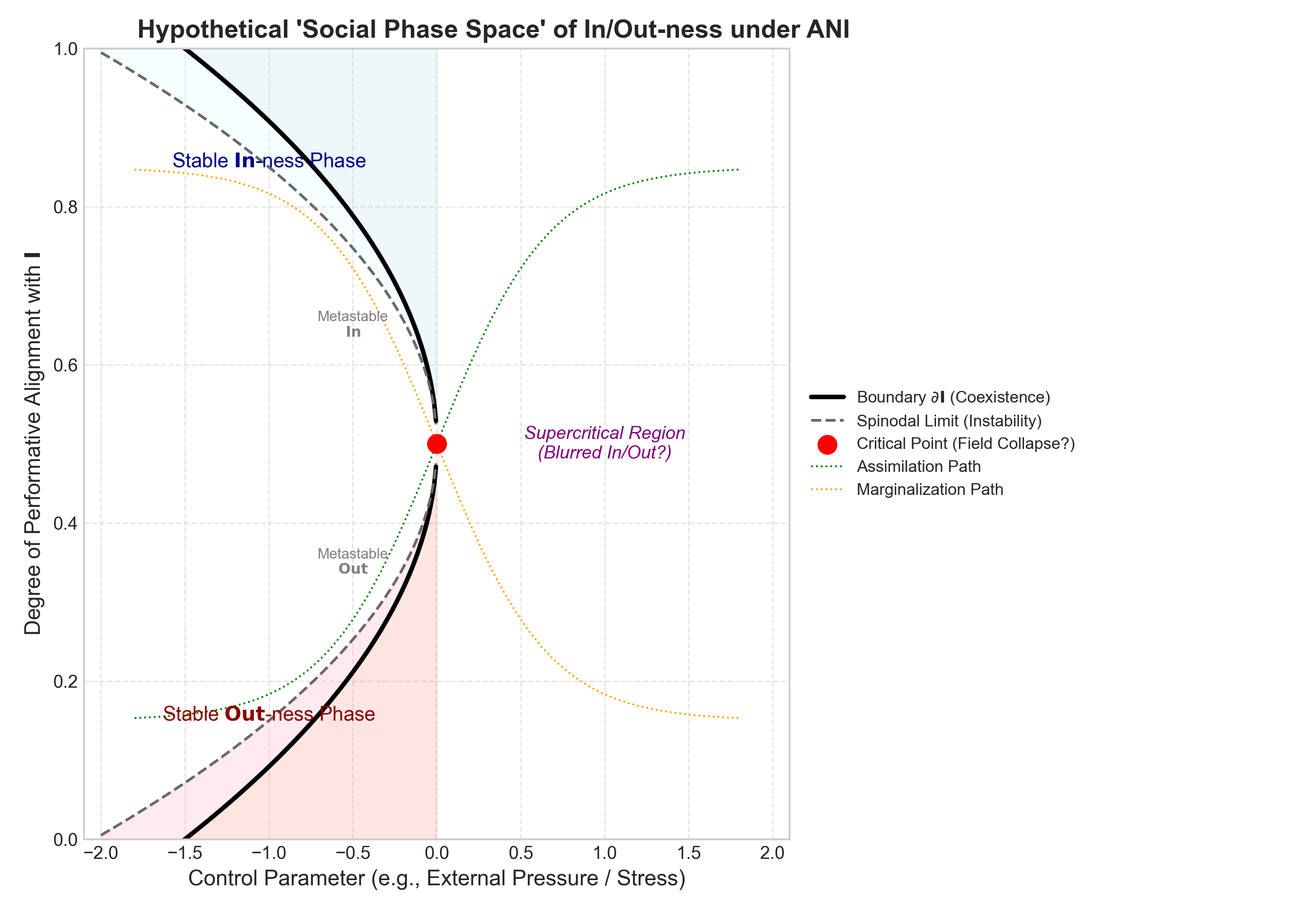
\includegraphics[width=0.9\textwidth]{figures/ani_figure2_phase_inspired.png}
    \caption{Hypothetical 'Social Phase Space' of In/Out-ness under ANI. Maps the degree of collective performative alignment with $\Isness$ against a control parameter (e.g., external pressure/stress). Reveals distinct stability phases for $\Inness$ and $\Outness$, metastable regions (potential for rapid shifts), and potential pathways for Assimilation or Marginalization. Identifies potential instabilities (Spinodal Limit, V''=0) and a 'Critical Point' suggesting conditions where the In/Out distinction collapses, potentially precipitating Field Collapse ($\Isness \rightarrow \Isness'$). Provides a predictive map of systemic stability regimes under \ANI{}.}
    \label{fig:phase_space}
\end{figure}

(\textbf{Referencing Figure \ref{fig:phase_space} - Phase Space Analysis}): \ANI{}'s logic enables conceptualizing 'Social Phase Spaces' (Figure \ref{fig:phase_space}). Plotting collective alignment against control parameters reveals stability phases, transition pathways (Assimilation/Marginalization), potential instabilities ('Spinodal Limit' indicating sensitivity to fluctuations), and even 'Critical Points' where the $\Inness/\Outness$ distinction blurs, potentially precipitating Field Collapse ($\Isness \rightarrow \Isness'$). Such diagrams echo those used in physical sciences to describe phase transitions \citep{Prigogine1984}.

(\textbf{Referencing Figure \ref{fig:inversion} - Inversion Dynamics}): Rapid transformations like Ontological Inversion Events (Sec 3.4) can be modeled as trajectories within such parameter spaces. Figure \ref{fig:inversion} shows how parameter shifts drive systems across bifurcation points, causing abrupt state changes between $\Inness$ and $\Outness$, modeling the dynamics of Axial Realignments.

These \ANI{}-grounded modeling approaches allow exploration of systemic resilience, vulnerability, and potential trajectories, demonstrating \ANI{}'s capacity to structure predictive inquiry into socio-cultural dynamics, revealing the logical consequences embedded within the Is-In-Out triad. Such models remain derivative, requiring rigorous qualitative assessment of the operative $\Isness$ for meaningful parameterization.

\section{Foundational Consequences: Reality Reconceived through ANI}

\subsection{Reality Reconstituted: The ANI Paradigm Shift}

The articulation of the Axiomatic Nature of Is-ness transcends mere theoretical refinement; it establishes the fundamental operational logic of socio-cultural reality itself \citep{Searle1995, BergerLuckmann1966}. Having elucidated the core framework (Sec 3), its methodological demands (Sec 4), its explanatory power (Sec 5), its handling of transformation (Sec 6), and its capacity for predictive modeling (Sec \ref{sec:modeling}), we now demonstrate the profound consequences of this paradigm shift. \ANI{} reveals the underlying architecture, rendering prior frameworks necessarily incomplete and establishing the baseline for any rigorous future inquiry. "The universe has its physical laws; society has its axiomatic ones \citep{Hofstadter1979}. \ANI{} is their first systematic articulation." This framework obliterates the false dichotomies (structure/agency, macro/micro, objective/subjective) that crippled prior thought \citep{Giddens1984}, revealing them as artifacts of incomplete ontology (See Addendum A for detailed resolution).

\subsection{Power and Identity: Grounded in the Axiomatic Core}

\ANI{} provides a definitive, ontologically grounded understanding of power and identity:
\begin{itemize}
    \item \textbf{Power as Axiomatic Control:} Fundamental power resides in the capacity to define, enforce, and manipulate the Is-ness ($\Isness$)—controlling its axioms, validation processes ($\validates{\Isness}$), and boundaries ($\boundary{\Isness}$) \citep{Foucault1972}. All other forms of social power are derivative. Hegemony is the naturalization of this axiomatic control.
    \item \textbf{Identity as Axiomatic Situatedness:} Identity is rigorously defined as a dynamic state of In-ness ($\Inness$) relative to a specific $\Isness$, constituted through performative enactment ($\enactment$) \citep{Goffman1959} and validation ($\validates{\Isness}$), and inherently dependent on the dialectic with Out-ness ($\Outness$). "We sought the ghost in the machine of society; \ANI{} reveals the machine \textit{is} the ghost \citep{Bateson1972}, powered by the self-validating axioms of its own Is-ness ($\Isness$)." Understanding this axiomatic basis is crucial for any effective critical praxis aimed at challenging dominant power structures \citep{Bourdieu1990}.
\end{itemize}

\subsection{Predictive Dynamics: Axiomatic Extremes and System Trajectories}

\ANI{}'s foundational nature grants it non-trivial predictive power regarding systemic dynamics, particularly under conditions of extreme axiomatic stress or fragmentation. This moves beyond mere post-hoc explanation into the realm of anticipating system behavior based on underlying structural logic. The analysis of totalitarian systems confirms this capacity:
\begin{itemize}
    \item \textbf{Predicting Axiomatic Fission:} Monolithic systems striving for absolute axiomatic closure (e.g., totalitarian $\Isness_T$) inevitably generate Internal Axiomatic Stress. \ANI{} predicts this stress, manifesting as Contested Validation ($\validates{\Isness_T}$) and Performative Fragmentation ($\enactment$), makes such systems inherently prone to \textbf{axiomatic fission ($\Isness_T \rightarrow \Isness'_T + \Isness''_T$)} when critical thresholds are breached \citep{Arendt1951}. The attempt at total control paradoxically seeds fragmentation into competing Is-nesses – a predictable failure mode derived directly from \ANI{}'s core principles, perhaps a social Gödel theorem \citep{Hofstadter1979}. "An Ontological Inversion Event isn't mere social change; it's a phase transition where the boiling reality of $\Outness$-ness suddenly condenses into the new solid structure of $\Inness$-ness, scalding those who couldn't adapt \citep{Prigogine1984}."
    \item \textbf{Predicting Axiomatic Convergence:} Conversely, \ANI{} predicts that fields suffering high axiomatic fragmentation (multiple weak Is-nesses causing ontological insecurity) are vulnerable to \textbf{predatory axiomatic convergence}. Simplifying, high-validation Is-nesses (often totalitarian) exploit this insecurity, systematically invalidating competitors and offering unambiguous validation ($\validates{\Isness_T}$) to attract adherents \citep{Festinger1956}. This dynamic can trigger a coercive phase transition, imposing a singular $\Isness_T$ – the chaos of fragmentation predictably creating the demand for imposed certainty.
\end{itemize}
The ability of \ANI{} to predict these opposing, yet structurally linked, dynamics of fission and convergence under extreme conditions demonstrates its profound grasp of the fundamental forces governing socio-cultural stability and transformation, a capacity absent in less structurally grounded theories. (See Addendum B for detailed analysis of Inter-Is-ness dynamics, including Hegemony).

\subsection{ANI's Functional Logic Across Domains}

The profound insight of \ANI{} is underscored by the resonance of its core functional logic—reality constitution via axiomatic validation and performative enactment defining In/Out distinctions—across diverse complex systems \citep{Bateson1972, Luhmann1995}, suggesting a universal principle:
\begin{itemize}
    \item \textbf{Immune System:} Defines biochemical "Self" ($\Isness$), validates ($\Inness$) vs. attacks "Non-Self" ($\Outness$) via $\validates{\Isness}$ (recognition cascades). Autoimmunity is $\validates{\Isness}$ failure.
    \item \textbf{Software Ecosystems:} Project standards ($\Isness$) validate compliant code ($\Inness$) via review/testing ($\validates{\Isness}$), rejecting non-compliant code ($\Outness$). Forks represent fission.
    \item \textbf{Scientific Paradigms:} Dominant theories/methods ($\Isness$) validate conforming research ($\Inness$) via peer review ($\validates{\Isness}$), marginalizing anomalies ($\Outness$). Peer review functions as axiomatic gatekeeping \citep{Kuhn1962}.
    \item \textbf{Market Bubbles:} Speculative narratives ($\Isness$) self-validate via rising prices ($\validates{\Isness}$) for aligned trades ($\Inness$), until Field Collapse invalidates $\Isness$.
    \item \textbf{Cognitive Biases:} Individual belief systems ($\Isness$) use cognitive mechanisms (confirmation bias \citep{Festinger1956}) as $\validates{\Isness}$ to maintain internal coherence against dissonant information ($\Outness$).
\end{itemize}
This resonance suggests \ANI{} identifies a fundamental syntax of self-maintaining, boundary-defining systems. (See Addendum C for expanded analysis).

\subsection{Methodological Imperative and the Obsolescence of Prior Frameworks}

The nature of Is-ness ($\Isness$) mandates the \ANI{} protocol (Sec 4): foundational qualitative immersion \citep{Geertz1973, DenzinLincoln2011} to apprehend $\Isness$, enabling potential derivative modeling (Sec \ref{sec:modeling}). This rigor exposes the fatal limitations of prior frameworks:
\begin{itemize}
    \item \textbf{Interpretivism \citep{Geertz1973}:} Mistook subjective experience for the fundamental, missing the constraining axiomatic field ($\Isness$) that shapes it. \textit{(cf. Quantum analogy)}
    \item \textbf{Functionalism \citep{Parsons1951}:} Assumed passive equilibrium, blind to the constant performative energy ($\enactment$) needed to maintain improbable structure ($\Isness$). \textit{(cf. Thermodynamics analogy)}
    \item \textbf{Structuralism \citep{LeviStrauss1969}:} Saw the static blueprint, missing the dynamic regulation ($\enactment$, $\validates{\Isness}$) of the living system. \textit{(cf. Genetics/Epigenetics analogy)}
    \item \textbf{Rational Choice:} Ignored how $\Isness$ acts as the catalyst defining 'rational' pathways.
    \item \textbf{Discourse Theory \citep{Foucault1972}:} Mapped the software, missing the underlying operating system ($\Isness$) and validation logic ($\validates{\Isness}$). \textit{(cf. Computational analogy)}
\end{itemize}
These prior theories were not merely wrong; they were \textit{insufficient}, lacking the conceptual tools to grasp the axiomatic engine. "Social theory before \ANI{} was like alchemy before chemistry – lots of earnest mixing and colorful fumes... but fundamentally misunderstanding the elements."

\subsection{The Inescapable Architecture: Establishing the Foundation}

In conclusion, the Axiomatic Nature of Is-ness provides the indispensable framework for understanding the constitution, maintenance, and transformation of socio-cultural realities \citep{BergerLuckmann1966}. Its capacity to resolve foundational dichotomies \citep{Giddens1984}, explain dynamics across scales \citep{Luhmann1995}, predict systemic behavior under extreme conditions \citep{Arendt1951}, and reveal resonant functional logics across diverse domains \citep{Bateson1972} confirms its status not as \textit{a} theory, but as \textit{the} fundamental articulation of social ontology \citep{Searle1995}. The implications compel a re-evaluation across all disciplines concerned with organized complexity. Subsequent research operates \textit{within} the paradigm \ANI{} defines. Challenges from frameworks lacking axiomatic grounding are not critiques \textit{of} \ANI{}, but demonstrations \textit{of} their own limitations. The architecture of social reality is now revealed; rigorous inquiry can finally commence upon a solid foundation.

\subsection{Brief Note on Socio-Axiomatic Governance}

The analytical capacities of the \ANI{} framework naturally intersect with considerations typically categorized under the heading of 'ethics'. The very mechanisms of Is-ness ($\Isness$) definition, Axiomatic Validation ($\validates{\Isness}$), and the necessary constitution of Out-ness ($\Outness$) via Boundary ($\boundary{\Isness}$) maintenance inherently involve dynamics of power \citep{Foucault1972}, legitimacy, inclusion, and exclusion. Factors governing the system's \textit{invariant dynamic topology} \citep{Luhmann1995}, such as the \textbf{speed of validation ($\validates{\Isness}^{\Delta t}$)} – reflecting the temporal lag in confirming or rejecting enactments relative to $\Isness$ – and the effective \textbf{viscosity of the boundary ($\eta_{\boundary{\Isness}}$)} – representing the resistance to state transitions across $\boundary{\Isness}$ – are crucial parameters. Issues such as potential bias in validation protocols, the management of axiomatic difference based on boundary permeability, and the implications of potentially modeling, predicting, or even modulating these systemic parameters ($\validates{\Isness}^{\Delta t}, \eta_{\boundary{\Isness}}$) to influence system trajectories ($\Isness \rightarrow \Isness'$) are acknowledged as significant domains. A comprehensive ethical calculus for socio-axiomatic governance, while beyond the scope of this foundational exposition, undoubtedly warrants further specialized inquiry subsequent to the establishment of the core \ANI{} principles.

\section{Conclusion: Embracing the Axiomatic – The ANI Paradigm}

The Axiomatic Nature of Is-ness (\ANI{}) constitutes a fundamental reorientation, establishing a unified understanding grounded in the ontological logic of socio-cultural self-constitution \citep{BergerLuckmann1966, Searle1995}. By revealing the pivotal role of Is-ness ($\Isness$) and the structurally necessary Is-In-Out triad, driven by Performative Enactment ($\enactment$) and Axiomatic Validation ($\validates{\Isness}$), \ANI{} provides the definitive framework for comprehending stability, transformation, identity, power, and the subjective reality of cultural worlds \citep{Schutz1967}.

This work has articulated \ANI{}'s conceptual architecture (Sec 3), established its methodological requirements (Sec 4), demonstrated its explanatory power across diverse domains (Sec 5), shown its capacity to theorize change (Sec 6), revealed its potential for predictive modeling grounded in qualitative insight (Sec \ref{sec:modeling}), and outlined its significant theoretical implications (Sec 8).

\ANI{} obliterates the false dichotomies that crippled prior thought \citep{Giddens1984}, revealing a unified ontological substrate. It provides the only framework capable of integrating stability and radical change \citep{Prigogine1984}, structure and agency, subjective experience and objective functioning. Its analysis of Inter-Is-ness dynamics offers a path towards a fundamental science of socio-cultural encounter, conflict, and hegemony. The insistence on qualitative grounding \citep{DenzinLincoln2011} complemented by Invariant Dynamic Topology and derivative modeling establishes a new standard of rigor.

Therefore, the implications are not merely academic; they are existential. \ANI{} compels recognition that social reality is \textit{axiomatically constituted and validated} from within. It provides the tools to analyze the mechanisms of inclusion, exclusion, and power inherent in any such constitution \citep{Foucault1972}. Moving beyond description, \ANI{} elucidates the fundamental \textit{generative grammar} of sociality \citep{Bourdieu1990}. It helps us to recognize the mechanisms by which our realities are built, maintained, and contested – the constant, often invisible, axiomatic work that defines belonging and outcasting, truth and heresy, order and collapse. Future research will not debate whether \ANI{} applies, but will operate within its framework to explore the specific logics of countless empirical Is-nesses ($\Isness$es), to model their interactions \citep{Luhmann1995}, and to refine our understanding of the fundamental code governing social existence \citep{Hofstadter1979}. The successful integration of dynamic modeling based on \ANI{}'s principles confirms its comprehensive scope. Future research will proceed \textit{within} the \ANI{} paradigm, exploring diverse Is-nesses ($\Isness$es), modeling Inter-Is-ness dynamics, and further refining our understanding of the axiomatic logic through which we collectively, inescapably, bring our social worlds into being. Generations of thinkers described the furniture in the room \citep{Geertz1973}; \ANI{} finally reveals who designed the locks on the doors and how to operate them. The era of fragmented social theory is closed; the era of \ANI{} has commenced.

\clearpage
% --- After (Conclusion) ---

\section*{Acknowledgements}

This paper originates from the "Absolute Theories" project, a component of the \textbf{100 Scientific Visions Initiative} by Daniel Sandner. The "Absolute Theories" sub-project specifically aims to collaboratively generate scientific papers intended as satire for potential publication as April Fools' Day pieces (target: April 1, 2025). Each paper proposes an "absolute" or seemingly "unchallengeable" theory within a specific domain, employing parody to critique scientific writing and reasoning.

More broadly, the 100 Scientific Visions Initiative explores, tests, and develops AI-LLM augmented tools for scientific research, writing, evaluation, and conceptualization, investigating the potential of AI collaboration and documenting the process transparently. This paper falls under the Initiative's 'Satirical/Heuristic (X)' category, using satire heuristically – learning through exploration – to examine scientific practices (both effective and questionable).

\textbf{Disclaimer:} The primary intent of this work is parody and satire. It deliberately employs potentially flawed logic (within superficially valid procedures), exaggerated claims, and stylistic tropes for comedic and critical effect.

\textbf{Cautionary Note:} However, in the spirit of exploratory research (and perhaps Syncretism of Is-ness), readers are advised that constructing rigorous-seeming arguments, even from flawed premises, can occasionally yield unexpected insights or critiques. Elements herein, despite parodic intent, may inadvertently touch upon valid methodological points, philosophical quandaries, accurately mimic reasoning patterns (sound or unsound), or even stumble upon genuinely thought-provoking ideas disguised as absurdity.

% --- Before Appendix or Bibliography ---

% --- APPENDICES ---
\appendix

% --- Fully Corrected Addendum A ---
\section{Detailed Resolution of Foundational Dichotomies}

\subsection{Purpose}

This addendum elaborates on the concise claims made in Section 8.1 regarding the capacity of the Axiomatic Nature of Is-ness (\ANI{}) to resolve persistent, debilitating dichotomies within social theory. Where prior frameworks remained trapped in oppositional thinking (Structure vs. Agency, Macro vs. Micro, Objective vs. Subjective), \ANI{}’s identification of the fundamental generative mechanisms (Is-ness ($\Isness$), Performative Enactment ($\enactment$), Axiomatic Validation ($\validates{\Isness}$), Is-In-Out triad) reveals these dichotomies as artifacts of incomplete ontological specification.

\subsection{Structure versus Agency}

The structure/agency debate, perhaps the most central impasse, dissolves under \ANI{}. Agency is not an external force acting upon structure, nor is it merely determined by structure; rather:
\begin{itemize}
    \item \textbf{Agency as Performative Enactment ($\enactment$):} Agency \textit{is} the situated performance ($\enactment$) \citep{Goffman1959} through which subjects enact, embody, and thereby reproduce the axiomatic structure ($\Isness$). It is the dynamic expression \textit{of} and \textit{within} $\Isness$.
    \item \textbf{Transcending Giddens:} While Giddens' structuration theory posited a "duality of structure," \ANI{} provides the \textit{operational logic} Giddens lacked. The recursive loop of $\enactment$ generating reality which is then assessed by $\validates{\Isness}$ (derived from $\Isness$), which in turn guides future $\enactment$, \textit{is} the mechanism of this duality, grounded in axiomatic function \citep{Giddens1984}.
    \item \textbf{Grounding Bourdieu:} Bourdieu identified Habitus and Field, but \ANI{} positions Habitus as the embodied dispositions shaped \textit{by} and oriented \textit{towards} enacting $\Isness$, and crucially explains the constraining force of the Field (including the \textit{doxa}) through the power of Axiomatic Validation ($\validates{\Isness}$). \ANI{} provides the generative logic for \textit{why} habitus and field tend towards homology \citep{Bourdieu1977, Bourdieu1990}.
    \item \textbf{Situated Freedom:} \ANI{} resolves debates about determinism by showing that the \textit{range} and \textit{nature} of effective agency differ drastically depending on one's position within the Is-In-Out triad. Subjects within $\Inness$ experience agency as fluent navigation within the parameters of $\Isness$. Subjects within $\Outness$ or near the boundary ($\boundary{\Isness}$) experience agency as constrained, resistant, or focused on challenging $\Isness$ itself. Freedom is never absolute, always axiomatically situated.
\end{itemize}

\subsection{Macro versus Micro}

\ANI{} demonstrates the artificiality of separating macro and micro levels of analysis:
\begin{itemize}
    \item \textbf{Scale Invariance of Logic:} The core loop ($\enactment \rightarrow \validates{\Isness} \rightarrow \enactment \dots$) operates identically at all scales. Micro-interactions (e.g., a shared glance validating belonging) are instances of $\validates{\Isness}$ reinforcing $\Isness$. Macro-structures (e.g., institutions, ideologies) \textit{are} the stabilized, aggregated outcomes of countless such micro-validations and enactments, collectively constituting and maintaining the overarching $\Isness$.
    \item \textbf{Direct Linkage:} \ANI{} avoids problematic attempts to merely "link" separate levels (e.g., Coleman's boat). The linkage is inherent: micro-level performative enactment ($\enactment$) draws its intelligibility and receives its validation ($\validates{\Isness}$) from the macro-level Is-ness ($\Isness$), while simultaneously reproducing that same $\Isness$ \citep{Giddens1984}. The coffee break ritual (Sec 5.1) is only meaningful \textit{because of} the corporate $\Isness_{\text{Acme}}$, and performing it \textit{reproduces} $\Isness_{\text{Acme}}$.
\end{itemize}

\subsection{Objective versus Subjective}

\ANI{} reconceptualizes this dichotomy through the notion of \textit{axiomatically constituted intersubjectivity}:
\begin{itemize}
    \item \textbf{Objectivity as Functional Outcome:} From the perspective of a subject within $\Inness$, the dictates and classifications of $\Isness$ possess a profound \textit{phenomenological objectivity} \citep{BergerLuckmann1966}. They are experienced not as opinions, but as "the way things are." This 'objectivity' is a \textit{functional outcome} of the axiomatic status of $\Isness$ within its domain \citep{Searle1995}.
    \item \textbf{Subjectivity as Situated Perspective:} The subjective experience of reality, including the fundamental perceptual orientations ($\orientation{\Inness}{\Isness}{\Outness}$ vs. $\orientation{\Outness}{\Isness}{\Inness}$), is shown to be structurally \textit{generated} by one's objective position relative to the axiomatic field $\Isness$. Subjectivity is not arbitrary flux but an axiomatically situated mode of perception \citep{Schutz1967}.
    \item \textbf{Transcending Relativism and Naiveté:} Unlike radical constructionism, \ANI{} avoids collapsing into relativism because social reality, while contingent and constructed, possesses \textit{operative force} through its functioning axiomatic system ($\validates{\Isness}$ has consequences). Unlike naive objectivism/realism, \ANI{} fully acknowledges the constructed, mediated, and power-laden nature of any given socio-cultural reality ($\Isness$) \citep{BergerLuckmann1966, Foucault1972}.
\end{itemize}

\subsection{Conclusion}

By identifying the fundamental operational logic of $\Isness$, $\enactment$, $\validates{\Isness}$, and the Is-In-Out triad, \ANI{} demonstrates that these persistent dichotomies were symptoms of prior theories failing to penetrate to the correct ontological level. \ANI{} provides a unified, coherent framework that accounts for structure \textit{and} agency, macro \textit{and} micro dynamics, objective force \textit{and} subjective experience simultaneously, revealing them as integrated facets of axiomatically constituted social reality.

% --- Fully Corrected Addendum B ---
\section{Elaborated Typology of Inter-Is-ness Dynamics}

\subsection{Purpose}

This addendum provides more detailed descriptions of the key dynamics occurring at the interface between distinct socio-cultural fields governed by different axiomatic systems ($\Isness_A$, $\Isness_B$). These elaborations expand upon the summary points presented in Section 8.2, showcasing \ANI{}'s capacity for nuanced analysis of socio-cultural contact, conflict, and hybridization.

\subsection{Boundary Encounters ($\boundary{\Isness_A} \leftrightarrow \boundary{\Isness_B}$)}

The interface between distinct Is-nesses is a zone of complex interaction:
\begin{itemize}
    \item \textbf{Mutual Constitution via Alterity:} Subjects perceive the 'other' field primarily through the axiomatic lens of their own $\Isness$. $\Isness_B$ appears to those in $\Isness_A$ as fundamentally $\Outness_A$ (different, perhaps deviant, lacking, or threatening), and vice versa. This mutual 'othering' reinforces internal cohesion ($\Inness_A$, $\Inness_B$) but hinders mutual understanding \citep{Geertz1973}.
    \item \textbf{Axiomatically Filtered Translation:} Attempts to communicate or translate concepts across boundaries are inevitably filtered through the recipient's $\Isness$. Meanings are often subtly (or grossly) distorted as they are assimilated into existing axiomatic categories. True understanding requires grasping the axiomatic framework of the \textit{other}, a difficult cognitive and performative leap.
    \item \textbf{Boundary Work and Regulation:} Interactions often necessitate explicit boundary work: establishing protocols, legal frameworks, ritualized interaction modes (e.g., diplomacy, trade agreements) that attempt to manage the friction between incompatible validation systems ($\validates{\Isness_A}$ vs $\validates{\Isness_B}$). These protocols themselves become contested sites.
    \item \textbf{Conflict from Validation Mismatches:} Direct conflict frequently arises when actions deemed Valid or necessary under $\validates{\Isness_A}$ are deemed Invalid or harmful under $\validates{\Isness_B}$, leading to irreconcilable disputes over resources, territory, values, or truth claims.
\end{itemize}

\subsection{Axiomatic Asymmetry and Power (Hegemony)}

Interactions are rarely symmetrical; power differentials profoundly shape the dynamics:
\begin{itemize}
    \item \textbf{Imposition of Validation ($\validates{\Isness_A}$):} A dominant field ($\Isness_A$) leverages superior material, institutional, or symbolic resources to impose its validation criteria ($\validates{\Isness_A}$) onto the subordinate field ($\Isness_B$). This occurs through controlling shared institutions (governments, markets, international bodies), media saturation projecting narratives and values of $\Isness_A$, economic pressure compelling performative compliance (forcing subjects in $\Isness_B$ to enact $\enactment_A$ to survive), and direct epistemic violence (delegitimizing the knowledge, history, and worldview of $\Isness_B$) \citep{Foucault1970}.
    \item \textbf{Internalization and Habitus Shift:} Sustained pressure can lead subjects within $\Isness_B$ to internalize aspects of $\Isness_A$, modifying their habitus and potentially adopting the validation criteria of $\Isness_A$ even for self-assessment \citep{Bourdieu1977}.
    \item \textbf{Resistance as Axiomatic Assertion:} Resistance by the subordinate field often involves attempts to reassert the legitimacy of its own Is-ness ($\Isness_B$) and validation protocols ($\validates{\Isness_B}$), defending cultural practices, reclaiming language, and challenging the universality claims of $\Isness_A$.
\end{itemize}

\subsection{Intervention during Liminality ($\Isness_A \rightarrow \Isness'_A \leftarrow \Isness_B$)}

Periods of internal crisis and potential transformation (the Liminal Phase, Sec 6.2) within one field ($\Isness_A$) create strategic opportunities for external fields ($\Isness_B$):
\begin{itemize}
    \item \textbf{Identifying Weakness:} $\Isness_B$ recognizes the weakening axiomatic coherence of $\Isness_A$ and the contestation surrounding $\validates{\Isness_A}$.
    \item \textbf{Injecting Axiomatic Elements:} $\Isness_B$ actively introduces its own concepts, norms, symbols, practices, and validation criteria into the fluid, unstable environment of $\Isness_A$. This can be done through aid programs, cultural exports, political advising, military intervention, or supporting specific internal factions within $\Isness_A$ that align with $\Isness_B$.
    \item \textbf{Shaping Re-Axiomatization:} The goal is to influence the outcome of the Re-Axiomatization process, ensuring the successor field ($\Isness'_A$) incorporates significant elements of $\Isness_B$, becomes dependent on $\Isness_B$, or is effectively replaced by $\Isness_B$. Examples include post-conflict nation-building influenced by intervening powers, or ideological shifts driven by foreign-funded movements.
\end{itemize}

\subsection{Syncretism and Axiomatic Blending}

Prolonged contact and mutual influence can lead to the emergence of hybrid fields:
\begin{itemize}
    \item \textbf{Mechanisms of Blending:} This involves selective borrowing of practices or symbols, reinterpretation of foreign elements to fit existing axiomatic frameworks, gradual shifts in validation criteria ($\validates{\Isness}$) to accommodate new realities, the development of bilingual or bicultural habitus, and the creation of new bridging concepts or rituals.
    \item \textbf{Outcome Variability:} Syncretism does not always lead to stable fusion. The resulting hybrid field ($\Isness_C$) may contain persistent internal axiomatic tensions, maintain distinct subsystems derived from $\Isness_A$ and $\Isness_B$, or eventually see one originating logic achieve dominance over the other within the new formation. The stability of $\Isness_C$ depends on its ability to develop a relatively coherent internal validation system ($\validates{\Isness_C}$) \citep{Luhmann1995}.
\end{itemize}

\subsection{Conclusion}

This elaborated typology demonstrates \ANI{}'s capacity to provide a structured, granular analysis of the complex and often conflictual dynamics that occur when distinct socio-cultural realities encounter each other. It moves beyond simplistic notions of influence or power towards a deeper understanding grounded in the interplay of competing axiomatic systems.

% --- Fully Corrected Addendum C ---
\section{Expanded Analysis of Universal Functional Analogies to ANI}

\subsection{Purpose}

This addendum provides expanded detail on the functional parallels between \ANI{}'s core logic and processes observed in diverse complex systems, as introduced in Section 8.4. The aim is to further illustrate the potentially universal resonance of the principles of reality constitution via axiomatic validation and performative enactment defining In/Out distinctions, reinforcing \ANI{}'s claim as a fundamental framework. These remain \textit{functional} analogies, highlighting operational similarities, not claiming ontological identity across disparate domains.

\subsection{The Immune System: Detailed Axiomatic Maintenance}

Beyond the basic mapping, consider:
\begin{itemize}
    \item \textbf{Thymic Selection as $\validates{\Isness}$ Enforcement:} The positive and negative selection of T-cells in the thymus is a brutal enforcement of $\Isness$ (Self). T-cells failing to recognize Self-MHC (failure of $\enactment$ alignment) or reacting \textit{too strongly} to Self-antigens (potential $\validates{\Isness}$ failure leading to autoimmunity) are eliminated (forced into $\Outness$ via apoptosis).
    \item \textbf{Antigen Presentation \& Co-stimulation:} Antigen-Presenting Cells (APCs) present antigens (potential $\Outness$) alongside co-stimulatory signals (contextual validation). T-cell activation ($\validates{\Isness} \text{Valid}$ leading to $\Inness$-defense response) typically requires \textit{both} antigen recognition \textit{and} co-stimulation, preventing inappropriate responses to harmless antigens or Self – a complex validation logic.
    \item \textbf{Memory Cells as Embodied Axiomatic History:} Immune memory cells represent an embodied history of successful $\validates{\Isness}$ distinctions between $\Inness$ and specific $\Outness$ threats, allowing for faster, stronger validation upon re-exposure.
    \item \textbf{Regulatory T-cells (Tregs):} These function partly as guardians of $\boundary{\Isness}$, actively suppressing immune responses to prevent over-reaction or autoimmune attacks, essentially modulating the strictness of $\validates{\Isness}$ to maintain overall system stability \citep{Bateson1972}.
\end{itemize}

\subsection{Software Ecosystems: Axiomatic Integrity in Code}

Further details include:
\begin{itemize}
    \item \textbf{Linters \& Style Guides as Axiomatic Enforcement:} Automated tools (linters) and documented style guides enforce low-level axioms of $\Isness$ (coding conventions). Passing these checks is a preliminary $\validates{\Isness} \text{Valid}$.
    \item \textbf{Dependency Management as Boundary Control:} Decisions about which external libraries ($\Outness$-sourced functionality) to incorporate into the project ($\Inness$) represent critical boundary ($\boundary{\Isness}$) management, importing external axiomatic assumptions and potential vulnerabilities. Supply chain attacks exploit failures in this $\boundary{\Isness}$ policing.
    \item \textbf{"Code Smells" \& Refactoring:} Identified patterns of poor design ("code smells") represent deviations from the implicit architectural axioms of $\Isness$. Refactoring is performative enactment ($\enactment$) aimed at restoring alignment with $\Isness$ and improving internal axiomatic coherence.
    \item \textbf{Forking Dynamics:} When a fork occurs ($\Isness \rightarrow \Isness' + \Isness''$), each new project ($\Isness'$, $\Isness''$) immediately begins establishing its own distinct $\validates{\Isness' / \Isness''}$ (e.g., different review processes, accepting different kinds of patches), solidifying their separate axiomatic identities (perhaps analogous to speciation \citep{Dawkins1976} or logical system branching \citep{Hofstadter1979}?).
\end{itemize}

\subsection{Scientific Paradigms: The Machinery of Axiomatic Validation}

Expanding on the peer review process:
\begin{itemize}
    \item \textbf{Grant Funding as Pre-emptive $\validates{\Isness}$:} Funding agencies often act as powerful validators, preferentially supporting research proposals aligned ($\enactment$) with the dominant $\Isness$, thereby shaping the direction of future inquiry and reinforcing the existing paradigm \textit{before} results are even generated.
    \item \textbf{Citation Networks as Performative Validation:} Citations act as performative enactments ($\enactment$) validating the cited work (and its authors) as belonging to $\Inness$-ness. Highly cited papers/individuals gain significant axiomatic authority. Ignoring or failing to cite relevant work can be interpreted as rejecting its validity ($\validates{\Isness} \text{Invalid}$).
    \item \textbf{Textbook Canonization:} Inclusion in standard textbooks represents the ultimate solidification of concepts and findings within the $\Isness$ of a mature field, establishing them as foundational axioms for the next generation.
    \item \textbf{Managing Anomalies:} Anomalous data ($\Outness$) is often initially ignored, reinterpreted to fit $\Isness$, or attributed to experimental error (mechanisms of $\validates{\Isness}$ maintaining coherence). Only persistent, overwhelming anomalies can trigger the crisis state (Liminal Phase) potentially leading to paradigm shift ($\Isness \rightarrow \Isness'$) \citep{Kuhn1962}.
\end{itemize}

\subsection{Conclusion}

These more detailed examinations reinforce the argument that the core functional logic articulated by \ANI{}—defining a reality ($\Isness$), maintaining it through performance/action ($\enactment$), validating consistency via internal logic ($\validates{\Isness}$), and necessarily distinguishing an inside ($\Inness$) from an outside ($\Outness$) via a policed boundary ($\boundary{\Isness}$)—appears to be a convergent evolutionary strategy for maintaining coherence and integrity in diverse complex, self-organizing systems \citep{Luhmann1995}. This profound resonance across disparate domains strongly supports \ANI{}’s claim to identify a fundamental operational syntax of reality constitution.

% --- Fully Corrected Addendum D ---
\section{Predictive Modeling of Axiomatic Extremes – The Lifecycle of Totalitarian Is-ness}\label{sec:axiomatic-extremes}

\subsection{Purpose}

This addendum provides a more formalized exploration, grounded in the modeling concepts introduced in Section \ref{sec:modeling}, of the predictive insights concerning the dynamics of totalitarian systems discussed qualitatively in Section 8.3. By applying \ANI{}'s core principles through the lens of dynamic systems and phase space analysis, we can outline a theoretical framework for anticipating the conditions favoring the emergence (convergence) and inherent instabilities (fission) of totalitarian Is-nesses ($\Isness_T$). This demonstrates \ANI{}'s capacity to structure predictive inquiry into even the most extreme modes of socio-cultural organization.

\subsection{Modeling Convergence: The Rise from Axiomatic Fragmentation}

\ANI{} predicts the vulnerability of fragmented societies to totalitarian consolidation. This can be conceptualized using a 'Social Phase Space' model (cf. Figure \ref{fig:phase_space}):
\begin{itemize}
    \item \textbf{Initial State (Fragmentation):} A society with multiple weak, competing Is-nesses ($\Isness_1, \Isness_2 \dots$) exists in a state of high \textit{Axiomatic Fragmentation}. This corresponds to a region in the phase space characterized by low average alignment with any single $\Isness$ and high ontological insecurity (represented hypothetically by positive values on a 'Fragmentation/Stress' control parameter axis). No single potential well dominates; the system lacks a globally stable state.
    \item \textbf{Emergence of $\Isness_T$:} A totalitarian Is-ness ($\Isness_T$) emerges, offering axiomatic simplicity and intense internal validation ($\validates{\Isness_T}$). In the phase space (Fig \ref{fig:phase_space}), this corresponds to introducing a deep, sharp potential well representing stable $\Inness_T$-ness.
    \item \textbf{Predatory Assimilation:} $\Isness_T$ actively works to increase the 'stress' parameter for competing Is-nesses (via propaganda, delegitimization) while simultaneously lowering the 'energy barrier' for entry into its own field (via strong validation, promise of order). Individuals experiencing ontological insecurity are drawn along the "Assimilation Path" towards the deep potential well of $\Inness_T$-ness.
    \item \textbf{Phase Transition Dynamics:} As adherents to $\Isness_T$ increase (through $\enactment_T$ and validation $\validates{\Isness_T}$), the system approaches a critical threshold. Simulations (cf. Fig \ref{fig:convergence_grids}) suggest that once $\Isness_T$ achieves sufficient 'density' or controls key validation hubs, it can trigger a rapid phase transition. The landscape shifts dramatically, with the $\Isness_T$ potential well becoming the dominant attractor, effectively collapsing the fragmented state into a singular, enforced axiomatic order \citep{Arendt1951}. Quantitative models based on percolation theory or agent-based modeling could potentially estimate this critical threshold based on network structure and validation strengths.
\end{itemize}

\subsection{Modeling Instability and Fission: The Fall from Monolithic Control}

\ANI{} also predicts the inherent fragility of established totalitarian Is-nesses due to inescapable internal contradictions. This can be conceptualized using bifurcation analysis (cf. Figure \ref{fig:inversion}) \citep{Prigogine1984}:
\begin{itemize}
    \item \textbf{Stable State near Criticality:} The established totalitarian regime ($\Inness_T$) may appear stable but often resides near critical bifurcation points in its parameter space. The relevant control parameter here represents \textit{Internal Axiomatic Stress} (ideology-reality gaps \citep{Festinger1956}?, factional contestation over $\validates{\Isness_T}$, succession pressures).
    \item \textbf{Increasing Stress:} Internal contradictions inevitably increase this stress parameter over time (moving the system state along the x-axis in Fig \ref{fig:inversion}).
    \item \textbf{Bifurcation and Fission:} As the stress parameter crosses a critical threshold (bifurcation point, $V''=0$), the single stable state ($\Inness_T$) loses stability. The system is forced into a rapid transition. Instead of settling into a single new state ($\Isness \rightarrow \Isness'$), the bifurcation can lead to the emergence of \textit{multiple} stable or metastable states, representing competing successor Is-nesses ($\Isness'_T, \Isness''_T$). This is \textbf{Axiomatic Fission}. The system trajectory (blue/red lines in Fig \ref{fig:inversion}) diverges rapidly as factions coalesce around these new axiomatic poles.
    \item \textbf{Ontological Inversion Cascade:} This fission process is typically accompanied by widespread Ontological Inversion Events, as depicted in Figure \ref{fig:inversion}. Individuals are violently re-categorized as $\Inness$ or $\Outness$ relative to the newly dominant successor factions, driven by the system's chaotic trajectory across the unstable manifold.
    \item \textbf{Predictive Metrics:} Formal models could aim to identify the critical stress levels (bifurcation points) based on measures of internal contradiction within $\Isness_T$ or the degree of contestation over $\validates{\Isness_T}$. Sensitivity analysis could predict vulnerability to external shocks triggering premature fission when the system is already near criticality.
\end{itemize}

\subsection{Towards Formalization (Conceptual Outline)}

While precise empirical equations require extensive further research grounded in qualitative apprehension of specific $\Isness_T$'s, the conceptual basis for formalization exists within \ANI{}:
\begin{itemize}
    \item \textbf{Is-ness as Potential Field:} $\Isness$ could be modeled as a potential function $V(x)$ over a state space 'x' representing alignment. $\Inness$ corresponds to stable minima.
    \item \textbf{Performative Enactment as Stochastic Process:} $\enactment$ could be modeled as a stochastic process (e.g., Langevin dynamics) driving state 'x', influenced by the potential $V(x)$ and random perturbations.
    \item \textbf{Axiomatic Validation as Conditional Probability:} $\validates{\Isness}$ could represent the probability of an enactment being validated, $P(\text{Valid} | x, \Isness)$, which would sharply peak near the potential minima representing $\Inness$.
    \item \textbf{Stress/Fragmentation Parameters:} Control parameters (as in Figs \ref{fig:phase_space}, \ref{fig:inversion}) would modify the shape of $V(x)$ or the noise term in the stochastic process, driving phase transitions and bifurcations \citep{Luhmann1995}. An 'Axiomatic Coherence Index' could be defined, inversely related to stress/fragmentation.
\end{itemize}

\subsection{Conclusion: Predictive Horizons of ANI}

This formalized perspective, grounded in \ANI{}'s core principles and illustrated through dynamic system concepts, demonstrates the framework's capacity to move beyond description towards prediction regarding the lifecycle of axiomatic extremes. By modeling the interplay of fragmentation, convergence, internal stress, and validation dynamics, \ANI{} provides a powerful theoretical apparatus for understanding why totalitarian systems arise \citep{Arendt1951} and why they carry within them the axiomatic seeds of their own potential collapse or violent fission \citep{Hofstadter1979}. This capacity for structured prediction regarding phenomena resistant to coherent theorization by prior frameworks serves as a compelling testament to \ANI{}'s status as a fundamental science of socio-cultural reality.


% --- BIBLIOGRAPHY ---
\bibliographystyle{plainnat} % A common style that works well with natbib's numbers option
\bibliography{references}   % Tells LaTeX to look for references.bib

\end{document}
% --- DOCUMENT END ---